\documentclass[11pt]{article}
\usepackage[margin=1.2in]{geometry}
\usepackage{amsmath,amssymb,amsthm}
\usepackage{tikz}
\usetikzlibrary{decorations.pathreplacing}
\usepackage[hidelinks]{hyperref}
\usepackage{enumitem}

\newtheorem{theorem}{Theorem}[section]
\newtheorem{lemma}[theorem]{Lemma}
\newtheorem{proposition}[theorem]{Proposition}
\newtheorem{corollary}[theorem]{Corollary}
\newtheorem{claim}[theorem]{Claim}
\theoremstyle{definition}
\newtheorem{definition}[theorem]{Definition}
\theoremstyle{remark}
\newtheorem{remark}[theorem]{Remark}
\newtheorem{example}[theorem]{Example}

\newcommand{\ACC}{\mathsf{ACC}^0}
\newcommand{\AC}{\mathsf{AC}^0}
\newcommand{\NC}{\mathsf{NC}^1}
\newcommand{\genus}{\gamma}
\newcommand{\layer}{\lambda}
\newcommand{\comp}{\circ}
\DeclareMathOperator{\lcm}{lcm}

\title{Constant-Width Circuits of Small Genus Compute Only $\ACC$ Functions}
\author{Alexey Milovanov}
\date{August 2026}
\hypersetup{
  pdftitle={Constant-Width Circuits of Small Genus Compute Only ACC0 Functions},
  pdfauthor={Alexey Milovanov}
}

\begin{document}
\maketitle

\begin{abstract}
We prove that every Boolean function computed by a polynomial-size layered circuit
of $\mathrm{AND}/\mathrm{OR}$ gates of constant computational width (only gates
count toward the width; input literals are unconstrained) whose underlying graph
has orientable genus $\mathrm{polylog}(n)$ lies in nonuniform $\ACC$. This resolves an
open question of Eric Allender~\cite{Allender23}, first claimed by Allender,
Datta and Roy in 2005 by an argument that was later found to be flawed and retracted; even the case of constant
genus $\ge 2$ had remained open. Combined with the converse direction, established by Hansen
for planar circuits, our result characterizes $\ACC$ as the class of functions
computed by constant-width polynomial-size circuits of bounded (indeed
polylogarithmic) genus.

The heart of the proof is a simple graph lemma: in any graph
that is layered (every edge joins consecutive layers), one can delete at most
$\genus(G)$ complete layers so that the remaining graph is planar; it combines a
discrete intermediate-value observation, the additivity of the orientable genus over
disjoint unions, and the piercing--packing duality for intervals. Unlike the 2005
approach, no embedding of the circuit into a surface is ever fixed, which is precisely how the argument avoids the error
that invalidated the earlier proof. The rest of the proof cuts the circuit at the
deleted layers into a polylogarithmic number of constant-width relations, evaluates
each planar piece in $\ACC$ by a width-reduction argument in the style of Hansen, and
composes the relations in constant depth.
\end{abstract}

\tableofcontents

%=====================================================================
\section{Introduction}\label{sec:intro}

\subsection{The problem and its history}\label{sec:history}

Barrington's celebrated theorem~\cite{Barrington89} identifies $\NC$ with the class of
languages recognized by constant-width polynomial-size branching programs, and its
proof runs through width-$5$ permutation programs, i.e.\ through the nonsolvable group
$S_5$. A long line of work has asked what happens to constant-width computation when
the \emph{topology} of the underlying graph is restricted, so that the group-theoretic
content of Barrington's construction becomes unavailable. Hansen \cite{Hansen03},
building on Hansen, Miltersen and Vinay~\cite{HMV02}, proved a clean answer for
planar topology:
\begin{quote}
constant-width polynomial-size \emph{planar} circuits compute exactly the functions in
$\ACC$.
\end{quote}
 This is a striking statement: planarity collapses the power of
constant-width circuits from $\NC$ down to $\ACC$, a class that is widely believed to be
strictly weaker, although no separation is known.

It is natural to ask how robust this collapse is. Allender, Datta and
Roy~\cite{ADR05} announced in 2005 that the collapse persists for circuits of
polylogarithmic genus.  Unfortunately, a key
geometric step is false, and the main result was retracted (we detail the specific failure of the 2005 argument in Section~\ref{sec:adr}).
In this paper we prove the statement for polylogarithmic genus, and in a
form that is stronger in one further respect: the width bound need only be imposed
on the gates of the circuit, not on its input literals.

\subsection{The model and the main theorem}\label{sec:mainthm}

Throughout, a \emph{layered circuit} is a finite directed acyclic graph whose vertices
are either \emph{literals} (an input variable $x_i$ or a negated variable $\lnot x_i$;
Boolean constants can be modelled as fan-in-$0$ gates) or \emph{gates} labelled
$\mathrm{AND}$ or $\mathrm{OR}$, together with a layer function
$\layer\colon V\to\mathbb{Z}_{\ge 0}$ such that every edge goes from a vertex of some
layer $i$ to a vertex of layer $i+1$, and literals have no incoming edges. Gates have
unbounded fan-in and fan-out; a fan-in-$0$ $\mathrm{AND}$ evaluates to $1$ and a
fan-in-$0$ $\mathrm{OR}$ to $0$. One gate is designated as the output. The
\emph{computational width} of the circuit is the maximum, over layers $i$, of the
number of \emph{gates} in layer $i$; literals are not counted, and any layer may
contain arbitrarily many literals. The \emph{underlying graph} of the circuit is the
simple undirected graph obtained by forgetting directions and labels, and
$\genus(C)$ denotes its orientable genus: the least integer $h$ such that the graph
embeds without crossings on a sphere with $h$ handles.

\begin{theorem}[Main Theorem]\label{thm:main}
Fix constants $w,s,k\in\mathbb{N}$ and $c>0$. Let $(C_n)_{n\ge 1}$ be a family of
layered circuits, where $C_n$ has $n$ input variables, at most $(n+1)^{s}$ vertices,
computational width at most $w$, and $\genus(C_n)\le c\,(\log_2 (n+1))^{k}$.
Then the family of Boolean functions computed by $(C_n)$ is in nonuniform $\ACC$:
there are constants $d$, $e$ and a finite set $M$ of moduli, depending only on
$(w,s,k,c)$, and a family of depth-$d$, size-$(n+1)^{e}$ circuits over unbounded
fan-in $\mathrm{AND}$, $\mathrm{OR}$, $\mathrm{NOT}$ and $(\mathrm{MOD}_m)_{m\in M}$
computing the same functions.
\end{theorem}

No uniformity is assumed of the circuit family, and none is claimed of the $\ACC$
family; this matches the nonuniform setting of~\cite{ADR05,Allender23}. The
special case of Theorem~\ref{thm:main} in which the width bound counts all vertices
(so that also the number of literals per layer is at most~$w$) is exactly the
statement of Open Question~3 of~\cite{Allender23}. Since genus is at most the
crossing number, we also obtain:

\begin{corollary}\label{cor:crossing}
Theorem~\ref{thm:main} holds verbatim with the genus bound replaced by the same bound
on the crossing number of the underlying graph.
\end{corollary}

Conversely, every $\ACC$ function is computable by constant-width polynomial-size
\emph{planar} (hence genus-$0$) layered circuits by Hansen's
Theorem~1~\cite{Hansen03}; Hansen's circuits use fan-in two, and a fan-in-two circuit
is a layered circuit in our sense. Together with Theorem~\ref{thm:main} this yields
the characterization: there is a constant $w_0$ (given by Hansen's construction) such that for every fixed $w\ge w_0$ and every genus bound
between $0$ and $\mathrm{polylog}$, constant-width polynomial-size layered circuits of
that genus compute exactly $\ACC$.

Two remarks on sharpness. First, the width restriction is essential: without it,
even planar circuits compute all of $\mathsf{P}$, by inserting planar crossover
gadgets at polynomial cost~\cite{Goldschlager77}. Second, extending the theorem to
genus $n^{\varepsilon}$, for any fixed $\varepsilon>0$, would imply
$\NC=\ACC$ by Barrington's theorem and a padding argument; the details are given
in Section~\ref{sec:open}. Thus the location of the transition between
$\mathrm{polylog}(n)$ and $n^{\varepsilon}$ remains open.

\subsection{Overview of the proof}\label{sec:overview}

The proof architecture is organized into four main stages. Below, we articulate the conceptual core of each stage, providing a level of detail that enables a specialist to grasp the complete mechanical workings of the proof. The full formal arguments follow in subsequent sections.

\subsubsection{Genus as a counter: the layer planarizer}\label{sec:ov-planarizer}

The single new graph-theoretic mechanism we introduce is the \emph{layer planarizer} (Theorem~\ref{thm:planarizer}):
\begin{quote}
\emph{Let $G$ be a finite graph equipped with a layer function $\layer\colon V(G)\to\mathbb{Z}$ such that every edge joins vertices of consecutive layers. Then there exists a set $P$ of at most $\genus(G)$ layers whose deletion (removing all vertices in these layers and their incident edges) leaves a planar graph.}
\end{quote}

We use the genus purely as a combinatorial counter for disjoint nonplanar subgraphs. Because the graph is layered, any connected nonplanar subgraph $H\subseteq G$ must meet every layer within its layer interval $I(H)=[\min_{v\in H}\layer(v),\,\max_{v\in H}\layer(v)]$. Consequently, connected nonplanar subgraphs with pairwise disjoint layer intervals are vertex-disjoint. By additivity of the orientable genus over disjoint unions \cite{BHKY62}, their number is bounded by $\genus(G)$. Thus the interval family $\{I(H) \mid H \text{ is a connected nonplanar subgraph}\}$ has packing number at most $\genus(G)$. Interval piercing--packing duality then gives a set $P$ of at most $\genus(G)$ layers that pierces every nonplanar witness, leaving a planar remainder.

\subsubsection{Proof architecture: reducing the circuit to relations}\label{sec:ov-relations}

Now we show how the layer planarizer is used to prove the Main Theorem. We first prune the circuit to remove all vertices that cannot reach the output gate. This pruning preserves the layered structure, does not increase the computational width or genus, and ensures that every surviving vertex functionally contributes to the output.

We then apply the layer planarizer to the pruned underlying graph to identify a set $P$ of at most $g := \genus(C_n)$ layers to delete. The pruning, the set $P$, and the resulting decomposition depend \emph{only} on the circuit topology and not on the input $x$. Therefore evaluation can be modeled as deterministic transitions between states in the constant-size space $Q = \{0,1\}^w$, parameterized by $x$. We call the transition from layer $i$ to layer $i+1$ \emph{exceptional} if either $i \in P$ or $i+1 \in P$. There are at most $2|P| \le 2g$ exceptional transitions.
The removal of the exceptional transitions partitions the remaining layers into at most $g+1$ contiguous intervals, which we call \emph{planar blocks}. By the planarizer lemma, the subcircuit induced by each block is planar.
This decomposition is \emph{half-open}: we never restore a deleted boundary layer to a planar block, because doing so could reintroduce nonplanarity (for example, a $K_{3,3}$ may lie between a layer of unboundedly many literals and the next gate layer). Keeping the interfaces separate preserves the planarity of every block. Example~\ref{ex:pipeline} illustrates the decomposition.

\begin{figure}[t]
\centering
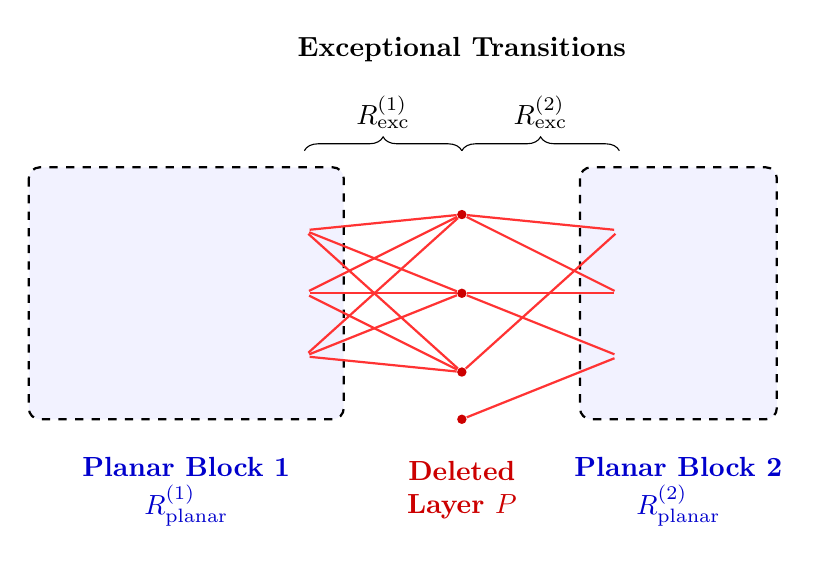
\begin{tikzpicture}[
    layer/.style={circle, fill=black, inner sep=1.2pt},
    planar edge/.style={thick, blue!80},
    exc edge/.style={thick, red!80},
    block/.style={rounded corners, draw, thick, dashed, fill=blue!5, inner sep=10pt}
]

% Planar Block 1
% Layer 1
\node[layer] (u1) at (0, 1.2) {};
\node[layer] (u2) at (0, 0.4) {};
\node[layer] (u3) at (0, -0.4) {};
\node[layer] (u4) at (0, -1.2) {};

% Layer 2
\node[layer] (v1) at (1.5, 0.8) {};
\node[layer] (v2) at (1.5, 0) {};
\node[layer] (v3) at (1.5, -0.8) {};

% Layer 3 (boundary of block 1)
\node[layer] (w1) at (3, 0.8) {};
\node[layer] (w2) at (3, 0) {};
\node[layer] (w3) at (3, -0.8) {};

% Draw planar edges inside Block 1
\draw[planar edge] (u1) -- (v1);
\draw[planar edge] (u2) -- (v1);
\draw[planar edge] (u2) -- (v2);
\draw[planar edge] (u3) -- (v2);
\draw[planar edge] (u3) -- (v3);
\draw[planar edge] (u4) -- (v3);

\draw[planar edge] (v1) -- (w1);
\draw[planar edge] (v2) -- (w2);
\draw[planar edge] (v3) -- (w3);
\draw[planar edge] (v1) -- (w2);

% Draw Block 1 box
\draw[block] (-0.5, 1.6) rectangle (3.5, -1.6);
\node[blue!80!black, font=\bfseries] at (1.5, -2.2) {Planar Block 1};
\node[blue!80!black] at (1.5, -2.7) {$R_{\text{planar}}^{(1)}$};

% Deleted Layer P
\node[layer, fill=red!80!black] (d1) at (5, 1) {};
\node[layer, fill=red!80!black] (d2) at (5, 0) {};
\node[layer, fill=red!80!black] (d3) at (5, -1) {};
\node[layer, fill=red!80!black] (d4) at (5, -1.6) {};
\node[red!80!black, font=\bfseries, align=center] at (5, -2.5) {Deleted\\Layer $P$};

% Planar Block 2
% Layer 5
\node[layer] (x1) at (7, 0.8) {};
\node[layer] (x2) at (7, 0) {};
\node[layer] (x3) at (7, -0.8) {};

% Layer 6
\node[layer] (y1) at (8.5, 1.2) {};
\node[layer] (y2) at (8.5, 0.4) {};
\node[layer] (y3) at (8.5, -0.4) {};
\node[layer] (y4) at (8.5, -1.2) {};

% Draw planar edges inside Block 2
\draw[planar edge] (x1) -- (y1);
\draw[planar edge] (x2) -- (y2);
\draw[planar edge] (x3) -- (y3);
\draw[planar edge] (x2) -- (y1);
\draw[planar edge] (x3) -- (y4);

% Draw Block 2 box
\draw[block] (6.5, 1.6) rectangle (9, -1.6);
\node[blue!80!black, font=\bfseries] at (7.75, -2.2) {Planar Block 2};
\node[blue!80!black] at (7.75, -2.7) {$R_{\text{planar}}^{(2)}$};

% Exceptional Edges (Crossing / Non-planar, demonstrating K3,3 complexity)
\draw[exc edge] (w1) -- (d1);
\draw[exc edge] (w1) -- (d2);
\draw[exc edge] (w1) -- (d3);

\draw[exc edge] (w2) -- (d1);
\draw[exc edge] (w2) -- (d2);
\draw[exc edge] (w2) -- (d3);

\draw[exc edge] (w3) -- (d1);
\draw[exc edge] (w3) -- (d2);
\draw[exc edge] (w3) -- (d3);

\draw[exc edge] (d1) -- (x1);
\draw[exc edge] (d1) -- (x2);
\draw[exc edge] (d2) -- (x2);
\draw[exc edge] (d2) -- (x3);
\draw[exc edge] (d3) -- (x1);
\draw[exc edge] (d4) -- (x3);

% Exceptional Relation braces
\draw [decorate,decoration={brace,amplitude=5pt,raise=6pt}]
  (3, 1.6) -- (5, 1.6) node [black,midway,yshift=20pt] {$R_{\text{exc}}^{(1)}$};

\draw [decorate,decoration={brace,amplitude=5pt,raise=6pt}]
  (5, 1.6) -- (7, 1.6) node [black,midway,yshift=20pt] {$R_{\text{exc}}^{(2)}$};

\node[font=\bfseries, align=center] at (5, 3.1) {Exceptional Transitions};

\end{tikzpicture}
\caption{Half-open decomposition of the circuit. The layers in $P$ are deleted; the intervening subcircuits are planar blocks (blue), while transitions incident to deleted layers are kept as exceptional relations (red). The circuit evaluates as $O \comp R_{\text{planar}}^{(2)} \comp R_{\text{exc}}^{(2)} \comp R_{\text{exc}}^{(1)} \comp R_{\text{planar}}^{(1)} \comp I_x$, with composition read right-to-left.}
\label{fig:planarizer_decomp}
\end{figure}

Consequently, evaluating the entire circuit reduces to the composition of at most $3g+1$ transition relations, plus two endpoint relations, i.e.\ at most $3g+3$ in total. To complete the proof of the Main Theorem, it suffices to establish the following three claims:
\begin{enumerate}
    \item \textbf{Planar Blocks:} The transition relation of any planar block of computational width $w$ can be evaluated in $\ACC$.
    \item \textbf{Exceptional Transitions:} For each of the constantly many pairs of states, deciding whether the transition maps one to the other is a single unbounded fan-in $\mathrm{AND}$/$\mathrm{OR}$ over literals, i.e.\ an $\AC$ predicate of $x$; no topological property is needed.
    \item \textbf{Composition:} The sequential composition of $O(g)$ such relations can be evaluated in constant depth $\ACC$ (relying on the fact that the genus $g$ is polylogarithmically bounded).
\end{enumerate}

Claim (2) is immediate, so Claims (1) and (3) complete the proof. The remainder of this overview outlines those two arguments.

\subsubsection{Planar blocks: generalizing the cylindrical upper bound}\label{sec:ov-planar-blocks}

To prove Claim (1)---that any planar block of width $w$ evaluates in $\ACC$---we use the \textbf{cylindrical upper bound} of Hansen, Miltersen and Vinay~\cite{HMV02,Hansen03}, quoted as Theorem~\ref{thm:hmv}. It states that any polynomial-size geometrically \emph{cylindrical} circuit (a layered circuit embeddable on a cylinder, or equivalently an annulus, without crossings) of fixed width can be evaluated by a constant-depth $\ACC$ circuit.

It cannot be applied directly: Hansen's upper bound requires bounded (binary) fan-in, whereas our planar blocks have arbitrary planar topology, unbounded fan-in gates, and an unbounded number of external input literals. We bridge this gap in two steps.

\paragraph{Step 1: Generalizing the upper bound to unbounded fan-in.}
First, we show that Hansen's theorem can be significantly strengthened: any cylindrical circuit with \emph{unbounded} fan-in can also be evaluated in $\ACC$. To achieve this, we must transform the circuit into a standard binary form without destroying its delicate cylindrical topology.

We extract an \emph{arc-order certificate} (see Lemma~\ref{lem:certificate})---a cyclic ordering of the arcs between consecutive layers dictated by the cylindrical embedding. We then binarize the circuit (Lemma~\ref{lem:binarize}) by replicating each arc, appending the necessary external inputs, and iteratively merging adjacent pairs of arcs using binary gates. Since only adjacent elements in the cyclic order are merged, the expanded circuit remains cylindrical. Its width --- now counting fresh input ports and $\mathrm{COPY}$ vertices --- grows by a factor of at most $w+1$, after which Theorem~\ref{thm:hmv} applies.

\paragraph{Step 2: Reducing planar blocks to cylinders via induction.}
With the unbounded-fan-in cylindrical case solved, we can finally prove Claim (1) by reducing arbitrary planar blocks to Step 1 (the formal induction is carried out in the proof of Theorem~\ref{thm:bridge}). We proceed by induction on the computational width $w$.

Let $o$ be a terminal gate of the planar block. We trace backward to find $a$, the first layer containing a gate that reaches $o$, and pick such a gate $v$. We define a computational cone $D$ as the set of all gates that lie on directed paths from $v$ to $o$.
The subcircuit $D$ is planar and layered, with unique source $v$ and unique sink $o$. By our other external ingredient, \textbf{Hansen's embedding theorem}~\cite[Theorem~2]{Hansen03}, every such digraph is \emph{cylindrical}.

The gates outside of $D$ form a residual circuit $R$. Because $D$ occupies at least one computational slot in every layer it spans, the computational width of $R$ is at most $w-1$. By induction, we can evaluate $R$ in $\ACC$.
We then simplify the interface: for every gate $g \in D$, we aggregate all of its incoming edges from outside $D$ (including literals and outputs from $R$) into a single fresh input bit $\beta_g$.

This leaves exactly the object handled in Step 1: a cylindrical block $D$ of width $w$, augmented with fresh inputs $\beta_g$, and unbounded fan-in. Applying Step 1 evaluates $D$ in $\ACC$, completing the induction and Claim (1).

\subsubsection{Composing polylogarithmically many relations}\label{sec:ov-compose}

Finally, to prove Claim (3), we must compose the $r \le 3g+3 = O(\mathrm{polylog}\, n)$ transition relations over the state space $Q$. This relies on a standard shallow divide-and-conquer technique well-known in circuit complexity (often used to show that reachability for short paths on bounded-width graphs is in $\AC$). The formal construction is detailed in Lemma~\ref{lem:compose}.

While a single relational composition costs merely an existential quantification over $Q$ (a constant fan-in $\mathrm{OR}$ of $\mathrm{AND}$s, which is essentially free in depth), composing $r$ relations naively would stack $r$ levels of logic, resulting in an unacceptable $\mathrm{polylog}(n)$ depth.

We circumvent this using a shallow divide-and-conquer strategy. We partition the sequence of $r$ relations into contiguous blocks of length $\lceil\log_2(n+1)\rceil$. To compose the relations within a single block, we existentially guess the intermediate state sequence. Since there are $|Q|^{\lceil\log_2(n+1)\rceil}$ possible sequences---which is polynomial in $n$ for constant $|Q|$---we can evaluate the composition in depth 2: a polynomial fan-in $\mathrm{OR}$ over all valid state sequences, followed by a fan-in-$\Theta(\log n)$ $\mathrm{AND}$ verifying the stepwise transitions.

This parallel composition reduces the sequence length from $r$ to $r / \lceil\log_2(n+1)\rceil$ at the cost of only $O(1)$ additional depth and polynomial size. Since the initial length $r$ is bounded by $O(\log^k n)$, applying this grouping recursively at most $k+1$ times collapses the entire sequence to a single relation. The total depth remains rigorously bounded by a constant, and the size remains polynomial. Applying this final relation to the designated input and output states resolves the circuit evaluation entirely within nonuniform $\ACC$. This establishes Claim (3) and completes the proof blueprint.

\subsection{Organization}

Section~\ref{sec:prelim} fixes the model. Section~\ref{sec:planarizer} proves the
layer planarizer theorem. Section~\ref{sec:cutting} performs the decomposition into
relations. Section~\ref{sec:bridge} proves the planar-block theorem
(Theorem~\ref{thm:bridge}), including the cylindrical binarization.
Section~\ref{sec:composition} composes the relations and completes the proof of
Theorem~\ref{thm:main}. Section~\ref{sec:adr} compares the method with the
retracted argument of~\cite{ADR05} and discusses open questions; Appendix~\ref{sec:formal}
describes the Lean~4 formalization.

%=====================================================================
\section{Preliminaries}\label{sec:prelim}

This section establishes the foundational models, definitions, and external theorems that will be used throughout the paper. We assume basic familiarity with Boolean circuits and graph theory.

\subsection{Layered Circuits and Graph Genus}\label{sec:model}

\paragraph{Layered Circuits.}
We recall the layered circuit model defined in Section~\ref{sec:mainthm} and fix the remaining conventions. A \emph{layered directed graph} (or layered digraph) has its vertex set partitioned into disjoint sets $V_0, V_1, \dots, V_h$, called \emph{layers}, such that every directed edge goes from some layer $V_\ell$ to the next layer $V_{\ell+1}$. This structure inherently prohibits cycles and antiparallel edges; we also assume there are no multiple edges between any pair of vertices. Negation occurs only at literals; there are no internal $\mathrm{NOT}$ gates. A literal evaluates to its value under $x$; an $\mathrm{AND}$ gate evaluates to the conjunction of the values of its predecessors in the previous layer ($1$ if it has none) and an $\mathrm{OR}$ gate to their disjunction ($0$ if it has none); the induction on the layer index is well founded because every predecessor of a layer-$\ell$ vertex lies in layer $\ell-1$.

\paragraph{Convention: Two notions of width.}
To avoid confusion, we explicitly distinguish two notions of circuit width used in this paper:
\begin{itemize}
    \item \textbf{Computational width} (denoted $w$): The parameter bounded in our Main Theorem. It counts \emph{only the computation gates} ($\mathrm{AND}/\mathrm{OR}$) in a layer. Literal vertices do not count toward computational width.
    \item \textbf{Width} (denoted $W$): The standard notion used in the cylindrical results of \cite{Hansen03,HMV02}. It counts \emph{every vertex} in a layer, including gates, literals, and $\mathrm{COPY}$ vertices.
\end{itemize}

\paragraph{Graph Genus.}
When we study the planarity and embeddings of the underlying graphs of these circuits, we rely on the topological concept of the \emph{orientable genus}. For a finite undirected graph $H$, its orientable genus, denoted $\genus(H)$, is the minimum number of ``handles'' that must be added to a sphere so that the graph can be drawn on the resulting surface without any of its edges crossing. For example, a sphere has genus $0$, a torus has genus $1$, and so on.

In this paper, we require three fundamental properties of the genus function $\genus$:
\begin{enumerate}
    \item \textbf{Planarity equivalence:} $\genus(H) = 0$ if and only if $H$ is a planar graph.
    \item \textbf{Monotonicity:} If $H'$ is a subgraph of $H$, then $\genus(H') \le \genus(H)$. Intuitively, deleting edges or vertices can only remove crossings.
    \item \textbf{Additivity over components:} For any graph $H$, its genus is exactly the sum of the genera of its connected components \cite{BHKY62}. If $H$ consists of disjoint pieces, their total topological complexity is simply the sum of the parts.
\end{enumerate}

\subsection{\texorpdfstring{$\ACC$}{ACC0} Circuits and Complexity Conventions}

The complexity class $\ACC$ ($\AC$ with counters) extends standard Boolean circuit classes by allowing counting modulo some integers. Formally, an $\ACC$ circuit family is a sequence of Boolean circuits (one for each input size $n$) that has \emph{constant depth} and \emph{polynomial size} (in $n$). The gates are allowed to have \emph{unbounded fan-in}, and they can be $\mathrm{AND}$, $\mathrm{OR}$, $\mathrm{NOT}$, as well as modular counting gates $\mathrm{MOD}_m$.

A $\mathrm{MOD}_m$ gate takes an arbitrary number of Boolean inputs and outputs $1$ if and only if the sum of its inputs (the number of $1$s) is a multiple of $m$. For any specific $\ACC$ circuit family, there must exist a fixed, finite set of moduli that are used across all circuits in the family.

In our reductions, we adopt the standard quantitative conventions, stated once here and then used silently. All circuit families discussed are nonuniform. Furthermore, local operations over a finite, fixed state space are considered ``free.'' Because any arbitrary Boolean function on a constant number of inputs can be computed by a constant-size truth-table circuit (i.e., Disjunctive Normal Form), these local operations can be substituted into an $\ACC$ circuit with only a constant blow-up in both depth and size.

When composing circuits, we do so by direct substitution: the total depth is bounded by the sum of the depths of the constituent circuits, and the size grows additively over each occurrence. If a subcircuit's result is used multiple times, we may either ``fan-out'' (reuse the physical subcircuit) or duplicate the subcircuit entirely, explicitly specifying our choice when size tracking is critical.

\subsection{Cylindrical Circuits}\label{sec:cyl}

To study highly restricted planar-like structures, we introduce the notion of \emph{cylindrical} embeddings. Mathematically, the cylinder is $S^1 \times \mathbb{R}$, where $S^1$ is the unit circle (representing the periodic width) and $\mathbb{R}$ represents the continuous length.

\begin{definition}[Layered Cylindrical Embedding]\label{def:cylindrical}
A \emph{layered cylindrical embedding} of a layered digraph maps the vertices
of each layer $V_\ell$ injectively to the circle $S^1\times\{\ell\}$.  Every
directed edge from $V_\ell$ to $V_{\ell+1}$ is represented by a simple
continuous arc in the closed annular strip between these circles.  The
interior of an arc is disjoint from all vertices, and interiors of distinct
arcs are disjoint; distinct arcs may meet only at a common endpoint.  In
particular, edges neither cross nor overlap.  Finally, every arc is \emph{monotone along the axis}: the axis coordinate increases strictly along the arc; equivalently, the arc is the graph of a continuous map from the axis interval $[\ell,\ell+1]$ to $S^1$.
\end{definition}

Monotonicity is part of the definition used in \cite{Hansen03,HMV02} --- there
all arcs are required to increase monotonically in the direction of the axis of
the cylinder --- and we keep it, both so that the theorems quoted below apply to
exactly the class defined here and because the sweep argument of
Lemma~\ref{lem:certificate} uses it.  It costs nothing: all cylindrical
embeddings we ever construct are built layer by layer with arcs drawn across a
single annular strip.

A layered digraph (or circuit) is called \emph{cylindrical} if there exists at least one such embedding. Unlike planarity, where vertices can be moved anywhere to avoid edge crossings, cylindricality forces vertices to remain strictly ordered on their respective layer circles (see Figure~\ref{fig:cyl_examples}).

\begin{figure}[t]
\centering
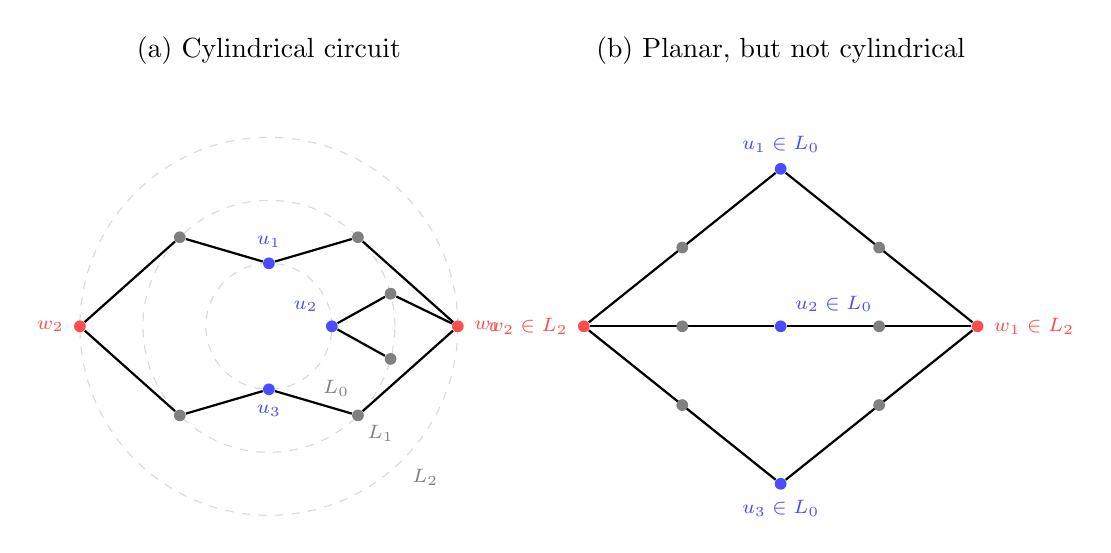
\begin{tikzpicture}[every node/.style={font=\scriptsize}]

% (a) Cylindrical circuit
\begin{scope}[shift={(0,0)}]
\node[font=\normalsize, anchor=south] at (0, 3.2) {(a) Cylindrical circuit};

% Draw concentric circles to show layers
\draw[gray!30, dashed] (0,0) circle (0.8);
\node[gray, below right] at (315:0.8) {$L_0$};
\draw[gray!30, dashed] (0,0) circle (1.6);
\node[gray, below right] at (315:1.6) {$L_1$};
\draw[gray!30, dashed] (0,0) circle (2.4);
\node[gray, below right] at (315:2.4) {$L_2$};

% L0 nodes (blue) - 3 nodes
\node[circle, fill=blue!70, inner sep=1.5pt, label={[blue!70]above:$u_1$}] (u1) at (90:0.8) {};
\node[circle, fill=blue!70, inner sep=1.5pt, label={[blue!70]above left:$u_2$}] (u2) at (0:0.8) {};
\node[circle, fill=blue!70, inner sep=1.5pt, label={[blue!70]below:$u_3$}] (u3) at (270:0.8) {};

% L2 nodes (red) - 2 nodes
\node[circle, fill=red!70, inner sep=1.5pt, label={[red!70]right:$w_1$}] (w1) at (0:2.4) {};
\node[circle, fill=red!70, inner sep=1.5pt, label={[red!70]left:$w_2$}] (w2) at (180:2.4) {};

% L1 nodes (gray) - 6 intermediate nodes
\node[circle, fill=black!50, inner sep=1.5pt] (v1) at (45:1.6) {};
\node[circle, fill=black!50, inner sep=1.5pt] (v2) at (135:1.6) {};
\node[circle, fill=black!50, inner sep=1.5pt] (v3) at (225:1.6) {};
\node[circle, fill=black!50, inner sep=1.5pt] (v4) at (315:1.6) {};
\node[circle, fill=black!50, inner sep=1.5pt] (v5) at (15:1.6) {};
\node[circle, fill=black!50, inner sep=1.5pt] (v6) at (345:1.6) {};

% Edges connecting u1, u3 to w1, w2 via L1
\draw[thick] (u1) -- (v1); \draw[thick] (v1) -- (w1);
\draw[thick] (u1) -- (v2); \draw[thick] (v2) -- (w2);
\draw[thick] (u3) -- (v3); \draw[thick] (v3) -- (w2);
\draw[thick] (u3) -- (v4); \draw[thick] (v4) -- (w1);
\draw[thick] (u2) -- (v5); \draw[thick] (v5) -- (w1);
\draw[thick] (u2) -- (v6); % No edge from v6 to w2!

\end{scope}

% (b) Planar but not cylindrical (K_3,2)
\begin{scope}[shift={(6.5,0)}]
\node[font=\normalsize, anchor=south] at (0, 3.2) {(b) Planar, but not cylindrical};

% L0 nodes (blue)
\node[circle, fill=blue!70, inner sep=1.5pt, label={[blue!70]above:$u_1 \in L_0$}] (a1) at (0, 2) {};
\node[circle, fill=blue!70, inner sep=1.5pt, label={[blue!70]above right:$u_2 \in L_0$}] (a2) at (0, 0) {};
\node[circle, fill=blue!70, inner sep=1.5pt, label={[blue!70]below:$u_3 \in L_0$}] (a3) at (0, -2) {};

% L2 nodes (red)
\node[circle, fill=red!70, inner sep=1.5pt, label={[red!70]right:$w_1 \in L_2$}] (c1) at (2.5, 0) {};
\node[circle, fill=red!70, inner sep=1.5pt, label={[red!70]left:$w_2 \in L_2$}] (c2) at (-2.5, 0) {};

% Draw paths
\draw[thick] (a1) -- (1.25, 1) node[circle, fill=black!50, inner sep=1.5pt] {} -- (c1);
\draw[thick] (a1) -- (-1.25, 1) node[circle, fill=black!50, inner sep=1.5pt] {} -- (c2);

\draw[thick] (a3) -- (1.25, -1) node[circle, fill=black!50, inner sep=1.5pt] {} -- (c1);
\draw[thick] (a3) -- (-1.25, -1) node[circle, fill=black!50, inner sep=1.5pt] {} -- (c2);

\draw[thick] (a2) -- (1.25, 0) node[circle, fill=black!50, inner sep=1.5pt] {} -- (c1);
\draw[thick] (a2) -- (-1.25, 0) node[circle, fill=black!50, inner sep=1.5pt] {} -- (c2);

\end{scope}

\end{tikzpicture}
\caption{Comparison of embeddings. (a) A cylindrical circuit drawn on concentric layer circles ($L_0$ blue, $L_2$ red). (b) The graph obtained by connecting the dangling gray vertex to $w_2$, redrawn in the plane. It is planar but not cylindrical: capping the three sources and the two sinks produces a layered digraph containing $K_{3,3}$, so Theorem~\ref{thm:hansen2} rules out a layered cylindrical embedding.}
\label{fig:cyl_examples}
\end{figure}

We specifically study \emph{standard} cylindrical circuits, restricted to use fan-in-two $\mathrm{AND}$ and $\mathrm{OR}$ gates, as well as fan-in-one $\mathrm{COPY}$ gates. Input vertices --- literals of formal variables, and constants --- may occur in \emph{any} layer, not only the first. We will need this latitude, because the binarization of Lemma~\ref{lem:binarize} creates fresh input vertices in intermediate layers. It is the convention of \cite{Hansen03,HMV02}: their circuits are layered digraphs whose input nodes ``can be literals or boolean constants'', with no restriction on the layer; \cite[Lemma~7]{HMV02} is devoted to constants in every layer but the first; and Hansen's own proof of his Theorem~1 inserts fresh input variables in intermediate layers.

Two closure properties of the geometric class will be used without further comment: a subgraph of a cylindrical layered digraph is cylindrical (restrict the embedding), and deleting or relabelling vertices and arcs never destroys cylindricality.



We rely on two landmark theorems regarding cylindrical circuits:

\begin{theorem}[{Hansen \cite[Theorem~2]{Hansen03}}]\label{thm:hansen2}
A layered digraph is cylindrical if and only if it is a subgraph of an acyclic planar layered digraph that possesses a unique source and a unique sink.
\end{theorem}

Theorem~\ref{thm:hansen2} bridges the geometric intuition of cylinder embeddings with the topological rigidity of planar graphs. The unique source and sink effectively ``cap'' the ends of the cylinder, allowing continuous deformation into a sphere, tightly controlling edge routing.

The second theorem demonstrates that narrow cylindrical circuits have low computational complexity. The width of a layered circuit is the maximum number of vertices in any single layer (recall that $W$ counts \emph{all} vertices, including input ports and $\mathrm{COPY}$ gates).

\begin{theorem}[{Hansen--Miltersen--Vinay \cite[Theorem~2]{HMV02}, quoted through \cite[Theorem~8 and Corollary~9]{Hansen03}}]\label{thm:hmv}
For every fixed integer maximum width $W$, there exist constants $d_W$, $e_W$, and a finite set of moduli $M_W$ satisfying the following property:

Let $D$ be any standard cylindrical circuit of width at most $W$ and total size $N$, whose inputs are literals of formal variables $y_1, \dots, y_m$ and constants. For any choice of up to $W$ designated output vertices in $D$, there exists an $\ACC$ circuit of depth at most $d_W$ and size at most $(N+1)^{e_W}$ over unbounded fan-in $\mathrm{AND}, \mathrm{OR}, \mathrm{NOT}$ and $(\mathrm{MOD}_m)_{m \in M_W}$ gates that computes the chosen outputs of $D$.
\end{theorem}

\begin{proof}[Derivation of the stated quantitative form]
Hansen's Corollary~9 says that for every fixed width $W$ and every polynomial size bound
$p$ there are a polynomial $q$ and a constant height $h$ such that every Boolean function
on $n$ inputs computed by a cylindrical circuit of width $W$ and size at most $p(n)$ is
computed by an $\ACC$ circuit of size $q(n)$ and depth $h$, over the finite modulus set
fixed by the construction for width $W$.  Three routine adjustments give the form stated
above.

\emph{Parameters.}  Apply the corollary with the size of the circuit itself as the
parameter.  The inputs of $D$ carry $m$ distinct formal variables, and $m\le N$ because
each of them occurs at an input vertex; adjoin $N-m$ further formal variables that are
never read, so that $D$ becomes a cylindrical circuit on exactly $N$ inputs whose size is
at most $N$.  Now Corollary~9 applies with the identity polynomial $p(t)=t$ and yields a
polynomial $q_W$ and a depth bound $h_W$ depending on $W$ alone, together with an $\ACC$
circuit of size $q_W(N)$ and depth $h_W$ computing the designated output from
$y_1,\dots,y_N$; the adjoined variables may be set arbitrarily.  Since $N\ge 1$, enlarging
an exponent turns $q_W(N)$ into $(N+1)^{e_W}$.

\emph{Input vertices in intermediate layers.}  In \cite{Hansen03,HMV02} a cylindrical
circuit is a layered digraph of fan-in-two $\mathrm{AND}/\mathrm{OR}$ vertices and
fan-in-one $\mathrm{COPY}$ vertices whose input vertices carry literals or Boolean
constants, with no restriction on the layer they occupy; Hansen's own proof of his
Theorem~1 inserts fresh input variables in intermediate layers, and
\cite[Lemma~7]{HMV02} is devoted to constants in every layer but the first.  So the
latitude we need is already part of the quoted statement.

\emph{Several outputs.}  Corollary~9 is stated for one output.  Given at most $W$
designated vertices, apply it to the subcircuit ending at each of them --- a subgraph of
$D$, hence again cylindrical --- and run the resulting circuits in parallel; this changes
only a constant depending on $W$.
\end{proof}

The result behind Corollary~9 is \cite[Theorem~2]{HMV02}: circuit evaluation is reduced
to the word problem of a finite monoid attached to the width, whose groups are solvable,
and Barrington--Th\'erien~\cite{BT88} places the word problem of such a monoid in
$\ACC$.  We use that theorem only in the form quoted above, as Hansen states it for
geometrically cylindrical circuits; see Remark~\ref{rem:hmv-predicate}.

\begin{remark}[Why we use the geometric definition]\label{rem:hmv-predicate}
The paper \cite{HMV02} also prints a pairwise combinatorial predicate for
cylindricality, but at shared endpoints it is not equivalent to the geometric
definition.  For example, the geometrically cylindrical arcs
$1\to1$, $2\to1$, $3\to3$ fail the printed condition: the pair
$(1{\to}1,2{\to}1)$ would force vertex $3$ to connect only to $1$.
We therefore use neither that predicate nor the intermediate monoid constructed
from it.  Throughout this paper, ``cylindrical'' means the geometric class of
Definition~\ref{def:cylindrical}.  Hansen \cite{Hansen03} states both quoted
results for this class, including his restatement of \cite[Theorem~2]{HMV02} as
Theorem~8.  The only combinatorial data we extract from an embedding is the common
arc order of Lemma~\ref{lem:certificate}, obtained directly from the geometry.
\end{remark}

To summarize, the passage from planar circuits to $\ACC$ in Section~\ref{sec:bridge}
rests on exactly two external results---Theorems~\ref{thm:hansen2}
and~\ref{thm:hmv}---and uses only their statements.  The proof as a whole uses one
further external ingredient, the additivity of the orientable genus over components
\cite{BHKY62}, in Section~\ref{sec:planarizer}; Hansen's converse
construction~\cite[Theorem~1]{Hansen03} is used only for the characterization recorded in
Section~\ref{sec:mainthm}, not in the proof of Theorem~\ref{thm:main}.

% The notation table below is currently disabled; re-enable it (together with the
% \subsection heading) if a summary of symbols is wanted.
% \subsection{Notation Table}\label{sec:notation}
% For convenient reference, we summarize the frequently used notation in Table~\ref{tab:notation}.
% \begin{table}[hbp]
% \centering
% \begin{tabular}{ll}
% \hline
% \textbf{Symbol} & \textbf{Meaning} \\
% \hline
% $w, W$ & Computational width (gates only) and width (all vertices)\\
% $N, n$ & Total vertices in a circuit, and number of input variables\\
% $g$ & Orientable genus of the fixed circuit (in Section~\ref{sec:bridge} the letter $g$ denotes a gate instead)\\
% $Q, \zeta$ & State space $\{0,1\}^w$, and anchor state $0^w$\\
% $\sigma_i, \pi_i$ & State vector at layer $i$, and gate-to-coordinate mapping\\
% $F^x_i$ & Transition relation from layer $i$ to $i+1$ on input $x$\\
% $P, X$ & Planarizing set of deleted layers, and exceptional transitions\\
% $\Gamma_i, L_i$ & Set of computation gates, and set of literals in layer $i$\\
% $a,b$ & First gate layer and output layer\\
% $E^{\mathrm{block}}_{s,t}$ & Planar-block relation\\
% $D, R$ & Cone of computation, and residual circuit\\
% $\mathrm{Anc}(h)$ & $h$ together with all of its ancestors (all lying in $R$)\\
% $\Lambda$ & The leaf-and-port layer\\
% $T$ & Block length in Lemma~\ref{lem:compose}\\
% $\beta_g$ & Evaluated function fed to gate $g$\\
% \hline
% \end{tabular}
% \caption{Summary of notation.}
% \label{tab:notation}
% \end{table}


\section{The layer planarizer}\label{sec:planarizer}

\begin{theorem}[Layer planarizer]\label{thm:planarizer}
Let $G$ be a finite graph and let $\layer\colon V(G)\to\mathbb{Z}$ be a function such that
for every edge $uv$ of $G$, the layers of its endpoints differ by exactly one, i.e., $|\layer(u)-\layer(v)|=1$. Then there exists
a set of integers $P\subseteq\mathbb{Z}$ with $|P|\le\genus(G)$ such that
$G-\layer^{-1}(P)$, the graph obtained by deleting all vertices whose layer belongs to $P$,
is planar.
\end{theorem}

\begin{proof}
For a connected subgraph $H\subseteq G$, write $I(H)\subseteq\mathbb{Z}$ for its
\emph{layer interval}: the set of all integers between $\min_{v\in V(H)}\layer(v)$ and
$\max_{v\in V(H)}\layer(v)$.

Every connected $H$ meets every layer in $I(H)$.  Indeed, a path in $H$ from a
minimum-layer vertex to a maximum-layer vertex changes the layer by $\pm1$ at each
edge and therefore cannot skip an intermediate integer.

Now suppose that $H_1,\dots,H_r$ are connected nonplanar subgraphs whose layer
intervals are pairwise disjoint.  The $H_i$ are then vertex-disjoint, and additivity
of orientable genus over components \cite{BHKY62}, together with monotonicity under
taking subgraphs, gives
\[
r = \sum_{i=1}^{r} 1 \;\le\; \sum_{i=1}^{r} \genus(H_i) \;=\; \genus\Bigl(\bigsqcup_{i=1}^r H_i\Bigr) \;\le\; \genus(G).
\]
Thus the family of integer intervals
$\mathcal{F} = \{I(H) \mid H\subseteq G \text{ is connected and nonplanar}\}$.
has packing number at most $\genus(G)$.  Apply the standard greedy piercing
algorithm for intervals: repeatedly choose a surviving interval with least right
endpoint, put that endpoint in $P$, and discard all intervals containing it.  The
intervals chosen by the algorithm are pairwise disjoint, so the preceding bound
shows that $|P|\le\genus(G)$; by construction, $P$ meets every interval in
$\mathcal{F}$.

If $G-\layer^{-1}(P)$ were nonplanar, one of its connected components $K$ would be
nonplanar.  Then $I(K)\in\mathcal{F}$ contains some $p\in P$, while connectedness
forces $K$ to contain a vertex in layer $p$.  This contradicts the deletion of
$\layer^{-1}(P)$, and proves that the remainder is planar.
\end{proof}

\begin{remark}
The bound is tight: place $g$ disjoint copies of $K_{3,3}$ in disjoint ranges of
layers.  Their union has genus $g$ by additivity, and making it planar requires
deleting a layer from each of the $g$ ranges.

Furthermore, the theorem and its proof apply to any integer ``layer'' structure on a graph where adjacent vertices take consecutive values; nothing specific to the circuits of the graph is required.
\end{remark}

%=====================================================================
\section{From a circuit to few relations}\label{sec:cutting}

Throughout this section, we fix one circuit $C=C_n$ from the family of Theorem~\ref{thm:main}. We write $N\le (n+1)^s$ for its number of vertices, $w$ for its computational width, and $g=\genus(C)\le c(\log_2(n+1))^k$ for the genus of its underlying graph.

Our goal is to decompose the computation into simpler relations, separating the
nonplanar transitions from planar blocks.  The next two sections evaluate these
relations in $\ACC$ and compose them.

\subsection{Pruning}\label{sec:pruning}

Before we begin our decomposition, we first clean up the circuit by removing any parts of the computation that are irrelevant to the final output (let $o$ denote the output gate).

We prune the circuit by deleting every vertex from which there is no directed path to the output $o$. Why is this a safe and useful operation?
The values of all surviving vertices are unchanged: a deleted vertex cannot feed
into a survivor, since it would then have a path to $o$.
Second, the overall structure of the circuit is preserved or improved: the pruned circuit remains layered with the same layer function; its computational width does not increase; and because the underlying graph of the pruned circuit is a subgraph of the original one, its genus remains at most~$g$.

From now on, $C$ exclusively denotes the pruned circuit. In this pruned circuit, every vertex has a directed path to $o$, which importantly implies that the underlying graph is connected.

Let $a$ be the lowest index of a layer containing a gate, and let $b=\layer(o)$. Any directed path from a gate in layer $a$ to the output $o$ advances by one layer per step and, after its first vertex, contains only gates. Consequently, every layer $i \in [a,b]$ contains a gate, so $b-a+1 \le N$. Empty numerical gaps below $a$ or above $b$ are irrelevant and may be ignored.

\subsection{States and transitions}\label{sec:states}

To decompose the circuit into sequential relations, we need to formalize the notion of a ``state'' of the computation at any given layer. The challenge is that different layers might have different numbers of gates. We overcome this by defining a uniform state space.

For each layer $i$, let $\Gamma_i$ be its set of gates (since the computational width is $w$, we know $|\Gamma_i|\le w$) and $L_i$ be its set of literals. We choose (nonuniformly) an injective mapping $\pi_i\colon \Gamma_i\to\{0,\dots,w-1\}$. This mapping assigns each gate in layer $i$ to a unique coordinate index.

The \emph{state} of layer $i$ on a specific input $x$ is defined as the boolean vector $\sigma_i(x)\in Q:=\{0,1\}^{w}$. The coordinate $\pi_i(h)$ of this vector holds the evaluated boolean value of the gate $h$ under input $x$. All other coordinates, which do not correspond to any gate in $\Gamma_i$, are set to $0$; we call these \emph{dummy coordinates}. By doing this, we guarantee that all states across all layers live in the exact same uniform state space $Q$.

For any intermediate layer $a\le i<b$, the state of layer $i+1$ is entirely determined by the state of layer $i$ and the external input $x$. Specifically, for any $\mathrm{AND}$ gate $g \in \Gamma_{i+1}$, its value is the conjunction of its predecessors in layer $i$:
\[
\sigma_{i+1}(x)_{\pi_{i+1}(g)}
=\bigwedge_{\substack{h\in \Gamma_i\\ h\to g}} \sigma_i(x)_{\pi_i(h)}
\;\wedge\;
\bigwedge_{\substack{\ell\in L_i\\ \ell\to g}} \ell(x).
\]
(The formula for an $\mathrm{OR}$ gate is dual, replacing conjunctions with disjunctions.) All dummy coordinates of $\sigma_{i+1}$ are forced to $0$. Because the circuit is layered, the formula uses only the preceding layer.

We can abstract this logic into a transition function $F^x_i\colon Q\to Q$. This function is defined by the displayed formulas for \emph{all} vectors in $Q$, not just those that represent reachable, valid states of the circuit.

It is convenient to picture a relation on $Q$ (such as the graph of the function $F^x_i$) as a Boolean $|Q|\times|Q|$ matrix, and composition of relations is Boolean matrix multiplication in the same right-to-left order used above. Thus, the evaluation of the whole circuit is modeled as one long matrix product, and Lemma~\ref{lem:compose} computes such a product in constant depth by grouping the factors into blocks of logarithmic length.

To complete the picture, we introduce two endpoint relations to cleanly tie the beginning and end of the computation. We fix a universal anchor state $\zeta:=0^{w}\in Q$. We define two relations on $Q^2$: the initialization relation $I_x$, which holds for a
pair $(u,t)$ iff $u=\zeta$ and $t=\sigma_a(x)$, and the output relation $O$, which holds
for $(s,z)$ iff $z=\zeta$ and $s_{\pi_b(o)}=1$.  Let us look closer at $I_x$. The state $\sigma_a(x)$ is directly and easily computable: because $a$ is the minimal layer containing gates, each gate in layer $a$ has \emph{only} literal predecessors. Thus, computing $\sigma_a(x)$ simply requires evaluating at most $w$ coordinates, each of which is an unbounded fan-in $\mathrm{AND}$ or $\mathrm{OR}$ over literal values. Consequently, for any fixed pair of states $(u,t)\in Q^2$, deciding the relation $I_x(u,t)$ can be done by an $\AC$ function of the input $x$ (with size $O(w\cdot N)$ and constant depth). The final output relation $O(s,z)$ simply checks if the output gate's coordinate is $1$ and anchors to $\zeta$; it does not depend on the input $x$ at all.

By stringing these transitions together, the circuit $C$ evaluates to $1$ (accepts $x$) if and only if the following composed relation holds:
\[
\bigl(O\comp F^x_{b-1}\comp\cdots\comp F^x_{a}\comp I_x\bigr)(\zeta,\zeta).
\]
Here, we identify each function with its graph (as a binary relation), and composition is written right-to-left. Thus, $I_x$ is applied first, setting the initial state, followed by the chain of layer transitions, and finally filtered by $O$. If it happens that $a=b$, the middle sequence of transitions is empty, and acceptance is concisely expressed as $(O\comp I_x)(\zeta,\zeta)$.

\subsection{Cutting at the planarizing layers}\label{sec:halfopen}

Apply Theorem~\ref{thm:planarizer} to the underlying graph of the pruned circuit.
It gives a set of layers $P$ with $|P|\le g$ whose deletion leaves a planar graph.

We classify the transitions based on this set $P$. A transition index $i\in\{a,\dots,b-1\}$ (which corresponds to the transition between layer $i$ and $i+1$) is called \emph{exceptional} if either $i\in P$ or $i+1\in P$. Let $X$ denote the set of all exceptional indices. Any transition index not in $X$ is called a \emph{planar-block} index. Because each layer in $P$ can participate in at most two transitions (the one coming into it and the one leaving it), the number of exceptional transitions is bounded by $|X|\le 2|P|$.

\paragraph{Exceptional transitions are efficiently computable in $\AC$.}
Why do we separate exceptional transitions? Because even though they break planarity, they are structurally shallow. For any exceptional index $i$ and for any fixed pair of states $(s,t)\in Q^2$ (of which there are $4^w$), the condition that $F^x_i(s)=t$ can be checked by an $\AC$ function of the input $x$. To see why, hold $s$ fixed: computing each coordinate of $F^x_i(s)$ requires looking at the fixed bits of $s$, the constants, and the input literals $\ell(x)$, combining them via a single layer of unbounded fan-in $\mathrm{AND}/\mathrm{OR}$ gates. Checking if the result exactly equals the fixed vector $t$ is simply a conjunction of $w$ such coordinate equalities. This computation clearly fits in $\AC$ with size $O(wN)$ and constant depth.

\paragraph{Planar-block transitions.}
The planar-block indices naturally group themselves into maximal, contiguous integer intervals separated by the exceptional transitions. There are at most $|P|+1$ such intervals. Consider one such interval consisting of the transition sequence $F_{\alpha},\dots,F_{\beta-1}$.

Let us analyze the physical subcircuit used by this sequence of transitions. It involves the gates $\Gamma_{\alpha},\dots,\Gamma_{\beta}$ and the literals $L_{\alpha},\dots,L_{\beta-1}$. We claim that none of these layers lie in the deleted set $P$. Indeed, if there were some layer $j\in P$ such that $\alpha\le j\le\beta$, then one of the transitions touching $j$ (either $j-1$ or $j$) would have been classified as exceptional and placed in $X$, breaking the interval. Because this subcircuit $B$ relies exclusively on layers outside of $P$, its underlying graph is a subgraph of $G-\layer^{-1}(P)$. Since removing $P$ leaves a planar graph, $B$ itself is \emph{planar}. It is also properly layered, has computational width bounded by $w$, and contains at most $N$ vertices.

     This planar interval computes the composition $F_{\beta-1}\comp\cdots\comp F_{\alpha}$, capturing the input--output behavior of the subcircuit $B$ from the state at layer $\alpha$ to the state at layer $\beta$. We can isolate this behavior formally: for any fixed pair of states $(s,t)\in Q^2$, define a specialized circuit $B_{s}$. We form $B_{s}$ by taking $B$, deleting all incoming edges to the gates in $\Gamma_\alpha$, and forcing each gate $h\in \Gamma_\alpha$ to behave as the fixed boolean constant given by $s_{\pi_\alpha(h)}$ (realized by a fan-in-$0$ $\mathrm{AND}$ for $1$, and a fan-in-$0$ $\mathrm{OR}$ for $0$). Removing edges and relabeling vertices preserves the planarity, layeredness, and width bounds of $B$.

We then define the planar-block relation by declaring that $E^{\mathrm{block}}_{s,t}(x)$
holds iff the layer-$\beta$ state of $B_s$ under $x$ equals $t$.
(If $t$ requires a $1$ in a dummy coordinate at layer $\beta$, the relation is identically false.) Evaluating this relation therefore amounts to evaluating a conjunction of at most $w$ output bits from the planar circuit $B_s$. Section~\ref{sec:bridge} proves that this can be done in $\ACC$ with parameters depending only on $w$.

\begin{lemma}[Block relations are the block transitions]\label{lem:blockrel}
For every input $x$ and all $s,t\in Q$, $E^{\mathrm{block}}_{s,t}(x)$ holds if and only if $(F^x_{\beta-1}\comp\cdots\comp F^x_{\alpha})(s)=t$.
\end{lemma}
\begin{proof}
The proof is by induction on the layer index. For the state at layer $\alpha$ the claim holds by construction of $B_s$, because the gates of $\Gamma_\alpha$ are frozen to the coordinates of $s$ that they index and the dummy coordinates index no gate. If the layer-$j$ state of $B_s$ equals $(F^x_{j-1}\comp\cdots\comp F^x_\alpha)(s)$ then the same holds at layer $j+1$, since both sides are computed from the layer-$j$ values and the literals of layer $j$ by the same formulas, and both force dummy coordinates to $0$.
\end{proof}

\paragraph{The tally.}
Putting it all together, deciding if the circuit accepts $x$ boils down to evaluating the composition
$\bigl(O\comp R_x\comp I_x\bigr)(\zeta,\zeta)$. Here, $R_x$ is the composition of exceptional $\AC$ relations and planar-block relations in chronological order. The number of relational steps is at most $2|P|$ for the exceptional transitions, plus
$|P|+1$ for the planar blocks, plus $2$ for the endpoints $I_x$ and $O$, hence at most
$3g+3$ in total.

\begin{remark}[Why half-open blocks? The danger of restoring layers]\label{rem:k33}
A planar block must exclude every vertex of a deleted layer, so both transitions incident to that layer are exceptional.

It might be tempting to define planar blocks differently by ``restoring'' each deleted layer to the block on its immediate left or right, so that adjacent blocks cleanly meet at a shared boundary layer. However, this approach is fundamentally flawed: restoring a deleted layer can easily reintroduce crossing edges and destroy the planarity of the block (as visually demonstrated in the schematic of Figure~\ref{fig:planarizer_decomp}).

Accordingly, deleted layers are handled only through the exceptional $\AC$ relations (and at the boundaries through $I_x$ and $O$); those relations are evaluated algebraically and need not be planar.
\end{remark}

\begin{example}[The decomposition on a small circuit]\label{ex:pipeline}
Let $C$ have computational width $w=3$ and five layers:
\begin{itemize}
\item layer $0$: three literals $x_1,x_2,x_3$;
\item layer $1$: three $\mathrm{AND}$ gates $u_1,u_2,u_3$, with one edge $x_i\to u_i$ each;
\item layer $2$: three literals $x_4,x_5,x_6$ and one $\mathrm{OR}$ gate $c$, with edges
      $u_1,u_2,u_3\to c$;
\item layer $3$: three $\mathrm{OR}$ gates $v_1,v_2,v_3$, with all nine edges
      $x_4,x_5,x_6\to v_1,v_2,v_3$, and one further edge $c\to v_1$;
\item layer $4$: the output $\mathrm{AND}$ gate $o$, with edges $v_1,v_2,v_3\to o$.
\end{itemize}
Only gates count toward the width, so $w=3$, while layers $0$ and $2$ carry literals
freely. The underlying graph contains the $K_{3,3}$ formed by $\{x_4,x_5,x_6\}$ and
$\{v_1,v_2,v_3\}$, so $C$ is nonplanar.  It has genus $1$: the displayed $K_{3,3}$
embeds on a torus, and all remaining vertices attach without requiring another
handle.  The planarizer may take $P=\{3\}$.  Deleting layer $3$ destroys the
nonplanar core and leaves a forest.  (Deleting layer $2$ would work as well.)

Here $a=1$ is the first layer carrying a gate and $b=\layer(o)=4$, so the transition
indices are $1,2,3$. Since $3\in P$, the indices $2$ and $3$ are exceptional, and the
only planar-block index is $1$; the corresponding block is the subcircuit on layers $1$
and $2$, namely $u_1,u_2,u_3,c$ with the three edges into $c$, which is planar. The
states are $\sigma_1=(u_1,u_2,u_3)$, $\sigma_2=(c,0,0)$ --- two dummy coordinates, since
layer $2$ carries only one gate --- and $\sigma_3=(v_1,v_2,v_3)$,
$\sigma_4=(o,0,0)$. Writing $E^{\mathrm{block}}$ for the relation whose $(s,t)$ entry is
$E^{\mathrm{block}}_{s,t}$, acceptance is therefore decided by
\[
\bigl(O\comp F^x_{3}\comp F^x_{2}\comp E^{\mathrm{block}}\comp I_x\bigr)(\zeta,\zeta):
\]
one planar-block relation, two exceptional relations and the two endpoint relations,
five relations in all, within the bound $3g+3=6$.  The example also explains the
half-open convention: restoring layer $3$ to the block on its left would put the
$K_{3,3}$ back inside that block.
\end{example}

\subsection{Roadmap for the remaining proof}\label{sec:roadmap}
With the structural decomposition complete, the proof of Theorem~\ref{thm:main} now cleanly splits into two distinct tasks, which we resolve in the final two sections:
\begin{enumerate}
    \item \textbf{Evaluating the planar blocks (Section~\ref{sec:bridge}):} We must prove that each isolated planar block relation $E^{\mathrm{block}}_{s,t}$ can indeed be evaluated in $\ACC$ with parameters depending only on its width $w$. This is the mathematical core of the paper, achieved via induction on the computational width.
    \item \textbf{Composing the relations (Section~\ref{sec:composition}):} We must formally compose the alternating sequence of exceptional $\AC$ relations and planar-block relations. Since there are $O(\mathrm{polylog}\, n)$ such relations, we will use a shallow divide-and-conquer strategy to execute the full composition in constant depth, completing the proof.
\end{enumerate}
\section{Planar circuits of small computational width}\label{sec:bridge}

This section proves the main technical theorem of this paper: planar layered circuits of computational width $w$ can be evaluated in $\ACC$ with parameters depending only on $w$.\footnote{Throughout this section the letter $g$ denotes a gate; the genus does not appear, since all circuits considered here are planar.} As discussed in Section~\ref{sec:ov-planar-blocks}, this extends the upper-bound direction of \cite[Theorem~1]{Hansen03} (planar of constant width $\Rightarrow \ACC$) in two important ways: first, literals are unconstrained (they do not count toward the width, and there can be arbitrarily many per layer); second, the fan-in of the gates is unbounded.

The proof is by induction on the computational width $w$. Following Hansen's original insight, we view an output gate as the sink of a computational cone. The cone has width at most $w$, while its external inputs come from a residual circuit of width at most $w-1$. The main work is to preserve the planar and cylindrical structure through this decomposition.

\begin{theorem}[Planar bridge]\label{thm:bridge}
For every $w\ge 0$ there are constants $d_w$, $e_w$, $A_w$ and a finite modulus set $M_w$ such that the following holds. Let $B$ be a planar layered circuit with $N$ vertices and computational width at most $w$, and let $Z$ be a set of at most $w$ designated gates lying in one layer. Then there is a circuit of depth $\le d_w$ and size $\le A_w(N+1)^{e_w}$ over unbounded fan-in $\mathrm{AND},\mathrm{OR},\mathrm{NOT},(\mathrm{MOD}_m)_{m\in M_w}$ computing, simultaneously, the values of all gates in $Z$ as functions of the input variables.
\end{theorem}

\paragraph{Plan of the proof.} The proof proceeds by induction on $w$, following these four stages:
\begin{enumerate}
    \item Isolate the cone of computation.
    \item Aggregate the external interface.
    \item Binarize the cylindrical core.
    \item Assemble, using the induction hypothesis for the residual circuit.
\end{enumerate}

Applying Theorem~\ref{thm:bridge} to the block circuits $B_s$ of Section~\ref{sec:halfopen} with $Z=\Gamma_\beta$ yields all relations $E^{\mathrm{block}}_{s,t}$ with parameters depending only on $w$, as required for our main results (by Lemma~\ref{lem:blockrel}).

Before proceeding with the main induction, we establish two lemmas to convert a cylindrical digraph with unbounded fan-in into a standard form (fan-in-two and $\mathrm{COPY}$ gates) while preserving its cylindrical embedding. This conversion is necessary to apply the known cylindrical upper bound (Theorem~\ref{thm:hmv}). Lemma~\ref{lem:certificate} extracts a cyclic arc-order property from the embedding, which Lemma~\ref{lem:binarize} then uses to perform the conversion.


\begin{lemma}[Arc-order certificate]\label{lem:certificate}
Let $D$ be a layered digraph with a layered cylindrical embedding, and consider two consecutive layers $U$ and $V$ with an arc set $E$ directed from $U$ to $V$. The arcs between $U$ and $V$ exhibit perfect topological order.

Formally, there exist cyclic orders on the vertices of $U$ and on the vertices of $V$, and a single cyclic sequence $\Omega$ listing every arc of $E$ exactly once, such that:
\begin{enumerate}
    \item If you traverse the vertices of $U$ in their cyclic order, and for each vertex you list its outgoing arcs as a contiguous block (ordered appropriately), the concatenated result is exactly the cyclic sequence $\Omega$.
    \item If you traverse the vertices of $V$ in their cyclic order, and for each vertex you list its incoming arcs as a contiguous block, the concatenated result is again identically the cyclic sequence $\Omega$.
\end{enumerate}
Moreover, the cyclic order induced on any given layer is consistent---it matches the order used for the transition on its left and the transition on its right.
\end{lemma}

\begin{proof}
Fix the given layered cylindrical embedding of $D$. By definition, $U$ and $V$ are mapped to consecutive concentric circles on the plane, and the arcs of $E$ are disjoint simple curves contained in the annulus between them. For $t$ strictly between the two layer levels let $S_t$ be the intermediate circle at level $t$. By the monotonicity clause of Definition~\ref{def:cylindrical}, every arc meets $S_t$ in exactly one point, so reading these crossing points around $S_t$ lists every arc of $E$ exactly once; call the resulting cyclic sequence $\Omega_t$.

The sequence does not depend on $t$. Indeed, the crossing point of an arc with $S_t$ moves continuously in $t$, and two such points never collide, because distinct arcs are disjoint away from their endpoints; so $t\mapsto(\text{crossing points})$ is a path in the configuration space of $|E|$ distinct points of $S^1$, and that space has exactly one connected component per cyclic order. Write $\Omega$ for this common cyclic order.

Now let $t$ tend to the $U$-level. The crossing points of the arcs leaving a vertex $u\in U$ converge to $u$ itself, and the points of arcs leaving other vertices converge to those other vertices, which are distinct points of the $U$-circle. Hence for $t$ close enough to the $U$-level the out-arcs of each $u$ occupy a contiguous block of $\Omega$, and the blocks appear in the cyclic order of the vertices of $U$ on their circle; since $\Omega$ does not depend on $t$, this holds for $\Omega$ itself. Letting $t$ tend to the $V$-level gives, in the same way, that the in-arcs of each $v\in V$ form a contiguous block of $\Omega$, in the cyclic order of the vertices of $V$. Finally, the cyclic order a layer receives is in both cases the order of its vertices along its own circle, which is fixed by the embedding and therefore shared by the transition on the left and the transition on the right. Hansen constructs the same order inside the proof of his Theorem~2 (\cite[p.~6]{Hansen03}), but we do not need it: given the embedding, the order can be read off directly.
\end{proof}

\begin{figure}[t]
\centering
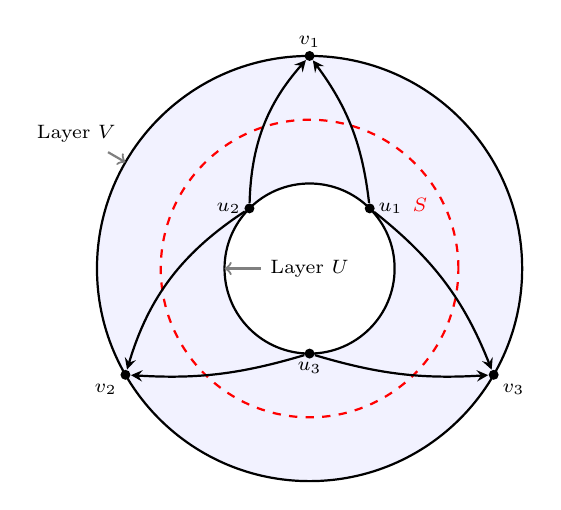
\begin{tikzpicture}[scale=0.9, every node/.style={font=\scriptsize}]
% Annulus boundaries
\draw[thick, fill=blue!5] (0,0) circle (3);
\draw[thick, fill=white] (0,0) circle (1.2);

% Labels for U and V
\node (labelV) at (150:3.8) {Layer $V$};
\draw[->, thick, gray] (labelV) -- (150:3);

\node (labelU) at (0,0) {Layer $U$};
\draw[->, thick, gray] (labelU) -- (180:1.2);

% Circle S
\draw[thick, dashed, red] (0,0) circle (2.1);
\node[red] at (30:1.8) {$S$};

% Vertices on U (inner)
\coordinate (u1) at (45:1.2);
\coordinate (u2) at (135:1.2);
\coordinate (u3) at (270:1.2);
\fill (u1) circle (2pt) node[right, inner sep=3pt] {$u_1$};
\fill (u2) circle (2pt) node[left, inner sep=3pt] {$u_2$};
\fill (u3) circle (2pt) node[below, inner sep=3pt] {$u_3$};

% Vertices on V (outer)
\coordinate (v1) at (90:3);
\coordinate (v2) at (210:3);
\coordinate (v3) at (330:3);
\fill (v1) circle (2pt) node[above, inner sep=3pt] {$v_1$};
\fill (v2) circle (2pt) node[below left, inner sep=3pt] {$v_2$};
\fill (v3) circle (2pt) node[below right, inner sep=3pt] {$v_3$};

% Edges U to V
\draw[thick, ->, >=stealth, shorten >=2pt, shorten <=2pt] (u1) to[bend right=15] (v1);
\draw[thick, ->, >=stealth, shorten >=2pt, shorten <=2pt] (u1) to[bend left=15] (v3);

\draw[thick, ->, >=stealth, shorten >=2pt, shorten <=2pt] (u2) to[bend left=20] (v1);
\draw[thick, ->, >=stealth, shorten >=2pt, shorten <=2pt] (u2) to[bend right=20] (v2);

\draw[thick, ->, >=stealth, shorten >=2pt, shorten <=2pt] (u3) to[bend left=10] (v2);
\draw[thick, ->, >=stealth, shorten >=2pt, shorten <=2pt] (u3) to[bend right=10] (v3);

\end{tikzpicture}
\caption{The arc-order certificate $\Omega$ is extracted by intersecting the planar arcs with a concentric circle $S$. Sliding $S$ inwards or outwards demonstrates that arcs leaving any $u \in U$ or entering any $v \in V$ must form contiguous blocks in the cyclic order, otherwise the planar embedding would be violated.}
\label{fig:annulus}
\end{figure}

\begin{lemma}[Combinatorial binarization]\label{lem:binarize}
Let $D$ be a layered digraph with a layered cylindrical embedding, having width at most $W_0$ and fan-in at most $F$. Let $N_D$ be the number of vertices in $D$. Assume each vertex $g$ carries a Boolean operation $\mathrm{op}_g\in\{\mathrm{AND},\mathrm{OR}\}$ and accepts one additional formal input $y_g$.

Then, $D$ can be transformed into a ``standard'' cylindrical circuit $D'$ over the inputs $(y_g)_g$ with the following properties:
\begin{enumerate}
    \item $D'$ uses only fan-in-two gates and $\mathrm{COPY}$ gates.
    \item $D'$ has width at most $(F+1)W_0$ and size $O_{F,W_0}(N_D)$.
    \item Each single layer of $D$ expands into at most $\lceil\log_2(F+1)\rceil+2$ layers in $D'$.
    \item For any assignment to the variables $y_g$, the specific vertex in $D'$ corresponding to $g\in D$ correctly evaluates to $\mathrm{op}_g$ applied to the set consisting of the values of the internal predecessors of $g$ together with $y_g$.
\end{enumerate}
\end{lemma}

\begin{proof}
The transformation proceeds transition by transition. We process every layer $V$ of $D$ alongside its incoming transition $U\to V$ (where $U$ is the preceding layer, or a virtual empty layer if $V$ is the first layer). The individual layer-by-layer constructions will be glued together at the layers of $D$, which we call \emph{checkpoints}. By Lemma~\ref{lem:certificate}, the cyclic order at a checkpoint is compatible with both its incoming and outgoing transitions.

Fix one such transition $U \to V$. Let $\Omega$ be the cyclic arc-order certificate guaranteed by Lemma~\ref{lem:certificate}. For each target gate $g\in V$, let $E_g$ denote the contiguous block of in-arcs to $g$ as they appear in $\Omega$. Since the fan-in is at most $F$, we have $|E_g|\le F$.

\emph{Cyclic matching principle.} If two consecutive layer circles carry finite sets of
vertices, and the endpoints of the arcs between them occur in the same cyclic order on
both circles, then the arcs can be drawn in the annulus pairwise disjointly and
monotonically along the axis. We use this in each of the three steps below, always with
an arc order inherited from $\Omega$.

\textbf{Step 1: Leaf-and-port layer.} We construct an intermediate layer $\Lambda$ directly after $U$. For every single arc $e=(u,g)$ in the transition, we create a $\mathrm{COPY}$ vertex $z_e$ in $\Lambda$, and draw an arc from $u$ to $z_e$. Additionally, for every gate $g\in V$, we introduce a fresh input vertex $p_g$ into $\Lambda$ that will carry the value $y_g$; this vertex has no incoming arcs.

We arrange $\Lambda$ cyclically by traversing $V$ and, for each $g$, laying out the block of its $\mathrm{COPY}$ vertices $z_e$ (for $e \in E_g$) followed immediately by $p_g$. By the cyclic matching principle, the arcs from $U$ to $\Lambda$ can be drawn without crossings.

\textbf{Step 2: Folding rounds.} The block for each gate $g$ in $\Lambda$ contains $|E_g|+1 \le F+1$ vertices. We want to apply the operation $\mathrm{op}_g$ to all of them. We do this by building a binary tree over $\lceil\log_2(F+1)\rceil$ rounds.

In each round, for every gate $g$, we take its current sequence of active vertices and pair them up adjacently. Each pair is fed into a new fan-in-two $\mathrm{op}_g$-gate (if there is an odd vertex left over, it passes through a $\mathrm{COPY}$ gate). For example, if $g$ has 3 incoming arcs, its initial sequence is $(z_1, z_2, z_3, p_g)$. Round 1 pairs them as $\mathrm{op}_g(z_1,z_2)$ and $\mathrm{op}_g(z_3,p_g)$. Round 2 pairs those two results into the final value (see Figure~\ref{fig:binarize} for an illustration of the full layer-by-layer folding process).

\begin{figure}[t]
\centering
\resizebox{\linewidth}{!}{
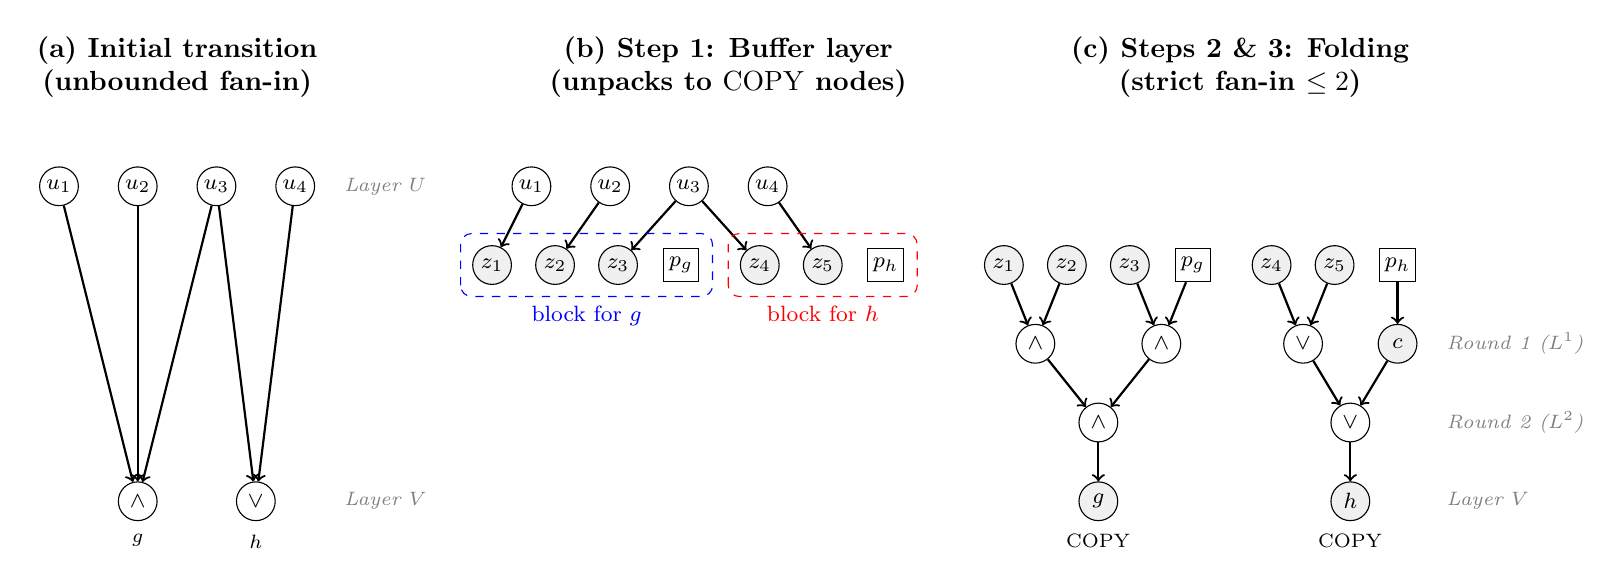
\begin{tikzpicture}[
  every node/.style={font=\footnotesize},
  v/.style={draw,circle,inner sep=1pt,minimum size=14pt},
  cp/.style={draw,circle,inner sep=1pt,minimum size=14pt,fill=black!6},
  port/.style={draw,rectangle,inner sep=2pt,minimum size=12pt},
  lbl/.style={anchor=south,font=\bfseries,align=center}]

  % PANEL A: Initial
  \begin{scope}[shift={(0,0)}]
    \node[lbl] at (1.5, 5) {(a) Initial transition\\(unbounded fan-in)};
    % Layer U
    \node[v] (u1) at (0, 4) {$u_1$};
    \node[v] (u2) at (1, 4) {$u_2$};
    \node[v] (u3) at (2, 4) {$u_3$};
    \node[v] (u4) at (3, 4) {$u_4$};
    \node[anchor=west,gray,font=\scriptsize\itshape] at (3.5, 4) {Layer $U$};

    % Layer V
    \node[v] (g) at (1, 0) {$\wedge$};
    \node[anchor=north,font=\scriptsize] at (1, -0.3) {$g$};
    \node[v] (h) at (2.5, 0) {$\vee$};
    \node[anchor=north,font=\scriptsize] at (2.5, -0.3) {$h$};
    \node[anchor=west,gray,font=\scriptsize\itshape] at (3.5, 0) {Layer $V$};

    % Edges
    \draw[->, thick] (u1) -- (g);
    \draw[->, thick] (u2) -- (g);
    \draw[->, thick] (u3) -- (g);
    \draw[->, thick] (u3) -- (h);
    \draw[->, thick] (u4) -- (h);
  \end{scope}

  % PANEL B: Step 1
  \begin{scope}[shift={(6,0)}]
    \node[lbl] at (2.5, 5) {(b) Step 1: Buffer layer\\(unpacks to $\mathrm{COPY}$ nodes)};
    % Layer U
    \node[v] (u1) at (0, 4) {$u_1$};
    \node[v] (u2) at (1, 4) {$u_2$};
    \node[v] (u3) at (2, 4) {$u_3$};
    \node[v] (u4) at (3, 4) {$u_4$};

    % Layer L0
    \node[cp] (z1) at (-0.5, 3) {$z_1$};
    \node[cp] (z2) at (0.3, 3) {$z_2$};
    \node[cp] (z3) at (1.1, 3) {$z_3$};
    \node[port] (pg) at (1.9, 3) {$p_g$};

    \node[cp] (z4) at (2.9, 3) {$z_4$};
    \node[cp] (z5) at (3.7, 3) {$z_5$};
    \node[port] (ph) at (4.5, 3) {$p_h$};

    % Edges
    \draw[->, thick] (u1) -- (z1);
    \draw[->, thick] (u2) -- (z2);
    \draw[->, thick] (u3) -- (z3);
    \draw[->, thick] (u3) -- (z4);
    \draw[->, thick] (u4) -- (z5);

    % Blocks
    \draw[dashed, blue, rounded corners] (-0.9, 2.6) rectangle (2.3, 3.4);
    \node[blue, anchor=north] at (0.7, 2.6) {block for $g$};

    \draw[dashed, red, rounded corners] (2.5, 2.6) rectangle (4.9, 3.4);
    \node[red, anchor=north] at (3.7, 2.6) {block for $h$};
  \end{scope}

  % PANEL C: Step 2 & 3
  \begin{scope}[shift={(12.5,0)}]
    \node[lbl] at (2.5, 5) {(c) Steps 2 \& 3: Folding\\(strict fan-in $\le 2$)};
    % Layer L0
    \node[cp] (z1) at (-0.5, 3) {$z_1$};
    \node[cp] (z2) at (0.3, 3) {$z_2$};
    \node[cp] (z3) at (1.1, 3) {$z_3$};
    \node[port] (pg) at (1.9, 3) {$p_g$};

    \node[cp] (z4) at (2.9, 3) {$z_4$};
    \node[cp] (z5) at (3.7, 3) {$z_5$};
    \node[port] (ph) at (4.5, 3) {$p_h$};

    % Layer L1
    \node[v] (a1) at (-0.1, 2) {$\wedge$};
    \node[v] (a2) at (1.5, 2) {$\wedge$};
    \node[v] (o1) at (3.3, 2) {$\vee$};
    \node[cp] (c1) at (4.5, 2) {$c$};
    \node[anchor=west,gray,font=\scriptsize\itshape] at (5.0, 2) {Round 1 ($L^1$)};

    % Layer L2
    \node[v] (rG) at (0.7, 1) {$\wedge$};
    \node[v] (rH) at (3.9, 1) {$\vee$};
    \node[anchor=west,gray,font=\scriptsize\itshape] at (5.0, 1) {Round 2 ($L^2$)};

    % Layer V
    \node[cp] (g) at (0.7, 0) {$g$};
    \node[anchor=north,font=\scriptsize] at (0.7, -0.3) {$\mathrm{COPY}$};
    \node[cp] (h) at (3.9, 0) {$h$};
    \node[anchor=north,font=\scriptsize] at (3.9, -0.3) {$\mathrm{COPY}$};
    \node[anchor=west,gray,font=\scriptsize\itshape] at (5.0, 0) {Layer $V$};

    % Edges L0->L1
    \draw[->, thick] (z1) -- (a1);
    \draw[->, thick] (z2) -- (a1);
    \draw[->, thick] (z3) -- (a2);
    \draw[->, thick] (pg) -- (a2);
    \draw[->, thick] (z4) -- (o1);
    \draw[->, thick] (z5) -- (o1);
    \draw[->, thick] (ph) -- (c1);

    % Edges L1->L2
    \draw[->, thick] (a1) -- (rG);
    \draw[->, thick] (a2) -- (rG);
    \draw[->, thick] (o1) -- (rH);
    \draw[->, thick] (c1) -- (rH);

    % Edges L2->V
    \draw[->, thick] (rG) -- (g);
    \draw[->, thick] (rH) -- (h);
  \end{scope}

\end{tikzpicture}
}
\caption{The three stages of the combinatorial binarization (Lemma~\ref{lem:binarize}) on one transition $U\to V$. (a) The original transition has unbounded fan-in. (b) The leaf-and-port layer replaces every arc by a $\mathrm{COPY}$ vertex and adds the fresh ports $p_g,p_h$; the arc-order certificate makes these contiguous noncrossing blocks. (c) Folding adjacent pairs produces binary trees and returns their values to the original checkpoint vertices, preserving both the cylindrical embedding and the checkpoint values.}
\label{fig:binarize}
\end{figure}

Because we only ever pair \emph{adjacent} elements within the contiguous block belonging to $g$, the cyclic order of the new layer matches that of the previous one, and the cyclic matching principle applies. After $r_0 = \lceil\log_2 (F+1)\rceil$ rounds, the sequence for each gate has collapsed to length 1.

\textbf{Step 3: Return to the checkpoint.} We add a final layer matching the original layer $V$, placing its vertices in their original cyclic order. Each gate $g$ receives one incoming arc from the root of its folding tree and is relabeled as a $\mathrm{COPY}$ gate. Since the binary tree has already computed $\mathrm{op}_g$, this $\mathrm{COPY}$ preserves the value needed by the next transition. The arcs to the final layer are drawn using the cyclic matching principle.

\textbf{Semantics and Complexity.} The binary tree computes $\mathrm{op}_g$ over all internal inputs plus the fresh input $y_g$. Because $\mathrm{AND}$ and $\mathrm{OR}$ are associative and commutative, this tree evaluates to exactly what $g$ would have computed. All arcs of the constructed embedding are drawn radially, hence are monotone along the axis, so the construction produces an embedding in the sense of Definition~\ref{def:cylindrical}.

The maximum size of $\Lambda$ is $\sum_{g\in V}(|E_g|+1) \le (F+1)W_0$. The folding rounds never increase the number of vertices, so no intermediate layer exceeds width $(F+1)W_0$. The total number of layers introduced per original transition is $1 (\text{for } \Lambda) + \lceil\log_2(F+1)\rceil (\text{rounds}) + 1 (\text{checkpoint}) = \lceil\log_2(F+1)\rceil+2$. Each vertex and each arc of $D$ contributes $O_{F,W_0}(1)$ vertices to $D'$, and a transition between two empty layers contributes none, so the total size is $O_{F,W_0}(N_D)$ as claimed. We do not pad the layers: Theorem~\ref{thm:hmv} is stated for width \emph{at most} $W$. (A reader who prefers the convention of \cite{HMV02}, where all layers carry the same number of vertices, may pad each layer in their way --- dummy input vertices in the first layer and dummy $\mathrm{COPY}$ vertices in the others --- which costs another $O_{F,W_0}(1)$ vertices per layer of $D'$, hence again $O_{F,W_0}(N_D)$ in total when $D$ has no empty layer, as is the case in our application.)
\end{proof}

\begin{proof}[Proof of Theorem~\ref{thm:bridge}]
The proof proceeds by induction on the computational width $w$.

\textbf{Base Case ($w=0$):} If $w=0$, the circuit contains no gates, so the designated set $Z$ is empty and the theorem holds.

\textbf{Inductive Step:} Assume $w \ge 1$. To simplify the notation, we first prove the theorem for a single designated output gate $o$.

Assume without loss of generality that all gates in $B$ can reach $o$ (any gates that cannot can be safely pruned, as discussed in Section~\ref{sec:pruning}). Let $a$ be the earliest layer containing a gate (of the pruned circuit). Pick an arbitrary gate $v$ in layer $a$.

\paragraph{Isolating the cone of computation.}

We partition the gates of $B$ into two sets: the \emph{cone} $D$, consisting of the gates
that lie on a directed $v\to o$ path, and the \emph{remainder} $R$, consisting of all
other gates of $B$. This partition has several critical structural properties:

\begin{enumerate}[label=(D\arabic*)]
\item\label{d:planar} $D$ is a planar, layered directed graph.
\item\label{d:source} $v$ is the unique source in $D$.
\item\label{d:sink} $o$ is the unique sink in $D$.
\item\label{d:everylayer} $D$ intersects every layer between $a$ and the layer of $o$.
\item\label{d:noexit} There are no arcs directed from $D$ to $R$.
\item\label{d:width} \textbf{(Crucial Width Reduction)} Because $D$ claims at least one gate in every layer (Property \ref{d:everylayer}), the residual circuit $R$ has computational width at most $w-1$.
\end{enumerate}

We record the proofs because the induction rests on these properties.
Throughout, ``$D$'' denotes the subdigraph of $B$ induced by the gate set $D$.

\ref{d:planar}: $D$ is an induced subgraph of $B$, and both planarity and the
layering are inherited by subgraphs.

\ref{d:source} and \ref{d:sink}: let $g\in D$, $g\ne v$, and fix a directed
$v\to o$ path through $g$.  Its predecessor of $g$ on that path is again a gate on a
$v\to o$ path, hence lies in $D$, so $g$ is not a source; symmetrically, if $g\ne o$
then its successor on that path lies in $D$, so $g$ is not a sink.  Conversely $v$
has no predecessor in $D$: a predecessor of $v$ inside $D$ would be a gate in layer
$a-1$, contradicting the minimality of $a$.
Likewise $o$ has no successor in $D$, since a successor
would lie on a $v\to o$ path strictly after $o$.

\ref{d:everylayer}: $v$ reaches $o$ --- this is exactly the pruning assumption ---
and a directed path in a layered digraph advances by exactly one layer per arc, so
it contains a vertex in every layer between $a$ and $\layer(o)$; all of these
vertices are gates, since literals have no incoming arcs, and all of them lie on a
$v\to o$ path, hence in $D$.

\ref{d:noexit}: suppose $g\in D$ and $g\to h$ with $h$ a gate of $B$.  By pruning,
$h$ reaches $o$, and $v$ reaches $g$; concatenating gives a $v\to o$ path through
$h$, so $h\in D$.  Thus no arc leaves $D$ for $R$.

\ref{d:width}: after pruning, every gate of $B$ lies in a layer between $a$ and
$\layer(o)$ --- gates above $\layer(o)$ cannot reach $o$, and there are no gates
below $a$ --- and by \ref{d:everylayer} each such layer contains a gate of $D$.
Since each layer of $B$ contains at most $w$ gates, each layer contains at most
$w-1$ gates of $R$.

By Properties \ref{d:planar}, \ref{d:source}, and \ref{d:sink}, $D$ is a planar layered digraph with a unique source and a unique sink. By Hansen's Theorem (Theorem~\ref{thm:hansen2}), applied to $D$ as a subgraph of itself, $D$ is cylindrical. We can therefore fix a valid layered cylindrical embedding for $D$. Note also that each layer of $D$ carries at most $w$ gates, so the \emph{internal} fan-in of $D$ --- the number of arcs a gate of $D$ receives from gates of $D$ --- is at most $w$, which is the exact condition needed for combinatorial binarization.

\begin{figure}[t]
\centering
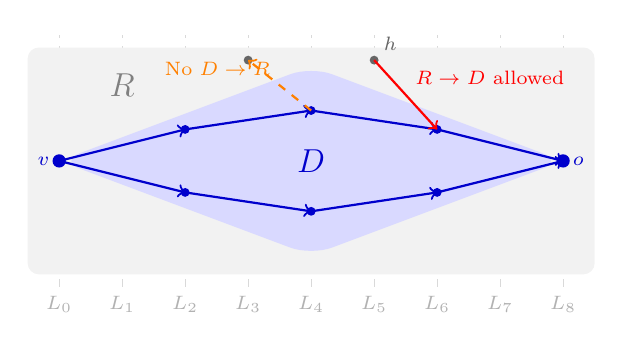
\begin{tikzpicture}[scale=0.8, every node/.style={font=\scriptsize}]
% Background grid to represent layers
\foreach \i in {0,...,8} {
    \draw[gray!30, dashed] (\i,-2) -- (\i,2);
    \node[gray!60, anchor=north] at (\i,-2) {$L_{\i}$};
}

% R area
\fill[gray!10, rounded corners] (-0.5,-1.8) rectangle (8.5,1.8);
\node[gray, font=\large\bfseries] at (1, 1.2) {$R$};

% D Cone area
\fill[blue!15, rounded corners=8pt] (0,0) -- (4,1.5) -- (8,0) -- (4,-1.5) -- cycle;
\node[blue!80!black, font=\large\bfseries] at (4, 0) {$D$};

% Source v and sink o
\fill[blue!80!black] (0,0) circle (3pt) node[left] {$v$};
\fill[blue!80!black] (8,0) circle (3pt) node[right] {$o$};

% Some nodes in D
\fill[blue!80!black] (2, 0.5) circle (2pt);
\fill[blue!80!black] (2, -0.5) circle (2pt);
\fill[blue!80!black] (4, 0.8) circle (2pt);
\fill[blue!80!black] (4, -0.8) circle (2pt);
\fill[blue!80!black] (6, 0.5) circle (2pt);
\fill[blue!80!black] (6, -0.5) circle (2pt);

% Some edges in D
\draw[->, thick, blue!80!black] (0,0) -- (2,0.5);
\draw[->, thick, blue!80!black] (0,0) -- (2,-0.5);
\draw[->, thick, blue!80!black] (2,0.5) -- (4,0.8);
\draw[->, thick, blue!80!black] (2,-0.5) -- (4,-0.8);
\draw[->, thick, blue!80!black] (4,0.8) -- (6,0.5);
\draw[->, thick, blue!80!black] (4,-0.8) -- (6,-0.5);
\draw[->, thick, blue!80!black] (6,0.5) -- (8,0);
\draw[->, thick, blue!80!black] (6,-0.5) -- (8,0);

% Some nodes in R
\fill[gray!80!black] (3, 1.6) circle (2pt);
\fill[gray!80!black] (5, 1.6) circle (2pt) node[above right] {$h$};

% Edge from R to D
\draw[->, thick, red] (5,1.6) -- (6,0.5);
\node[red, anchor=south west] at (5.5, 1.05) {$R \to D$ allowed};

% Invalid edge from D to R
\draw[->, thick, dashed, orange] (4,0.8) -- (3,1.6);
\node[orange, anchor=south east] at (3.5, 1.2) {No $D \to R$};

\end{tikzpicture}
\caption{Isolating the computational cone $D$ (Property \ref{d:width}). The cone spans every layer between its unique source $v$ and sink $o$ and occupies at least one gate in each layer. Hence the remaining circuit $R$ has computational width less than $w$. Edges may flow from $R$ into $D$, but never from $D$ to $R$.}
\label{fig:cone}
\end{figure}

\paragraph{Aggregating the external interface.}

We must now account for how $D$ interacts with the rest of the circuit. A gate $g \in D$ receives internal inputs from $D$ and external inputs from $R$ and raw literals.

We bundle all external inputs to $g$ (from $R$ and literals) into a single aggregated external input $\beta_g(x)$ using the same operation as $g$ ($\mathrm{AND}$ or $\mathrm{OR}$), with the usual convention in the empty case: if $g$ has no external inputs at all, then $\beta_g(x)=1$ for an $\mathrm{AND}$ gate and $\beta_g(x)=0$ for an $\mathrm{OR}$ gate, which is neutral for the operation of $g$. The final value of $g$ is then exactly its original operation applied to its internal inputs in $D$ together with $\beta_g(x)$.

For any external gate $h \in R$ that feeds into $D$, consider the subcircuit $\mathrm{Anc}(h)$ consisting of $h$ together with all of its ancestors (for $w=1$ the residual $R$ has computational width $0$, hence contains no gates at all, so no such $h$ exists and the case is vacuous). Property \ref{d:noexit} guarantees that no vertex in $D$ can reach $R$, meaning $\mathrm{Anc}(h)$ is entirely contained within $R$. Consequently, $\mathrm{Anc}(h)$ is a planar layered circuit of computational width at most $w-1$ (by Property \ref{d:width}).

By our inductive hypothesis, we can evaluate $\mathrm{val}_x(h)$ using an $\ACC$ circuit with parameters $(d_{w-1},e_{w-1},A_{w-1},M_{w-1})$, scaling as $A_{w-1}(N+1)^{e_{w-1}}$ in size.
To compute $\beta_g(x)$, we simply place one unbounded fan-in gate on top of the inductive $\ACC$ circuits for the $R$-predecessors and the raw literals. Summing over all $g \in D$, the total number of edges from $R$ (and from literals) into $D$ is bounded by the total number of edges in $B$, which is $O(N)$ since $B$ is planar. Therefore, we can compute all $\beta_g$ functions concurrently using $O\left(N \cdot A_{w-1}(N+1)^{e_{w-1}}\right)$ size.

\paragraph{Binarizing the cylindrical core.}

At this stage, the computation inside $D$ relies only on its internal edges and the aggregated external inputs $\beta_g(x)$ feeding into fresh formal inputs $y_g$. Since $D$ has at most $w$ gates per layer, the \emph{internal} fan-in of any gate $g \in D$ is at most $w$. Thus, even though $B$ has unbounded fan-in, $D$ has bounded internal fan-in, and Lemma~\ref{lem:binarize} applies with $W_0=w$ and $F=w$.

This yields a standard cylindrical circuit $D'$ containing only fan-in-two and $\mathrm{COPY}$ gates. The width of $D'$ is blown up slightly to $W(w) := (w+1)w$, and its total size is bounded by $O_w(N)$. The checkpoint vertices of $D'$ identically compute the values of the gates of $D$: by induction on the layer index, feeding $y_g := \beta_g(x)$ into $D'$ makes every checkpoint vertex of $D'$ evaluate to $\mathrm{val}_x(g)$, because the value of $g$ in $B$ equals $\mathrm{op}_g$ applied to its $D$-internal predecessors together with $\beta_g(x)$. The output $o$ corresponds to one specific checkpoint vertex in $D'$.

\paragraph{Assembling the induction step.}

Since $D'$ is a standard cylindrical circuit of bounded width $W(w)$ (where width $W$ counts all vertices, including input ports and $\mathrm{COPY}$ gates), we can invoke the cylindrical upper bound (Theorem~\ref{thm:hmv}). This yields an $\ACC$ circuit of depth $d_{W(w)}$ and size $\bigl(O_w(N)+1\bigr)^{e_{W(w)}}$ using moduli $M_{W(w)}$ that computes $\mathrm{val}(o)$ directly from the formal inputs $y_g$.

Finally, we compose the circuits. We take the $\ACC$ circuit for $D'$ and, into every formal input $y_g$, we wire the corresponding aggregated circuit for $\beta_g(x)$. The resulting combined circuit computes $\mathrm{val}_x(o)$ entirely from the original literals.

The final parameters are easily bound:
\begin{align*}
\mathrm{depth} &\le \underbrace{d_{W(w)}}_{\text{from } D'} + \underbrace{1}_{\text{aggregation gate}} + \underbrace{d_{w-1}}_{\text{from } R} =: d_w,\\
\mathrm{size} &\le \underbrace{\bigl(O_w(N)+1\bigr)^{e_{W(w)}}}_{\text{from } D'}
 + \underbrace{O\left(N \cdot A_{w-1}(N+1)^{e_{w-1}}\right)}_{\text{from } R} \;\le\; A_w (N+1)^{e_w}
\end{align*}
where $e_w := \max(e_{W(w)},\, e_{w-1}+1)$ and the moduli set is $M_w := M_{W(w)} \cup M_{w-1}$. All three of these final parameters depend exclusively on $w$.

To handle a full designated set $Z$ of up to $w$ gates, we repeat this construction for each gate in $Z$. This only affects the multiplier $A_w$, completing the induction and proving Theorem~\ref{thm:bridge}. No attempt is made to optimize $d_w$ and $e_w$; they inherit the non-explicit constants of the Barrington--Th\'erien theorem~\cite{BT88} through Theorem~\ref{thm:hmv}.
\end{proof}

%=====================================================================
\section{Composition, and the proof of the Main Theorem}\label{sec:composition}

We are now ready to assemble the final ingredients for our main result. In the previous sections, we saw how to break our original circuit evaluation into a sequence of relations (exceptional layers and planar blocks). The final step is to compose these relations. Since there are polylogarithmically many such relations, we need a way to compose them while maintaining constant depth and polynomial size.

\begin{lemma}[Constant-depth composition of polylogarithmically many
relations]\label{lem:compose}
Fix a finite set $Q$, an integer $A\ge1$, an integer $k\ge0$, a modulus set
$M$, and depth/size bounds $d_0$, $e_0$. Suppose $E^x_1,\dots,E^x_r\subseteq Q\times Q$
is a family of relations indexed by inputs $x\in\{0,1\}^n$ with $r\le A(\log_2(n+1))^{k}+A$.

Assume that for each $j$ and each pair $(s,t)\in Q^2$ the predicate
\[
x\;\longmapsto\;\bigl[\,(s,t)\in E^x_j\,\bigr]
\]
can be computed, on inputs of length $n$, by a circuit of depth $\le d_0$ and size
$\le(n+1)^{e_0}$ over the basis $\mathrm{AND},\mathrm{OR},\mathrm{NOT},
(\mathrm{MOD}_m)_{m\in M}$.

Then for $n$ larger than a
constant $n_0(A,k,|Q|)$, each predicate $x \mapsto [\,(s,t) \in (E^x_r\comp\cdots\comp E^x_1)\,]$ has such a circuit of depth $\le d_0+2(k+1)$ and
size $(n+1)^{e_1}$ with $e_1=e_1(e_0,|Q|,A,k)$, over the same modulus set $M$.
\end{lemma}

\begin{proof}
The goal is to compose $r$ relations into one, without blowing up the depth or size too much. We will do this in ``rounds''. In each round, we group consecutive relations into blocks and compose each block all at once.

To balance depth and size, we choose our block length to be $T=\lceil\log_2(n+1)\rceil$. We require $n$ to be large enough (i.e., $n>n_0$) so that $T\ge 2A$.

Consider a block of $\ell$ relations $E^x_{j+1},\dots,E^x_{j+\ell}$ where $\ell\le T$. To compute the composition of this block at a pair of states $(s,t)$, we ``guess'' the intermediate states. A path from state $s$ to state $t$ through these $\ell$ relations exists if and only if there is a sequence of intermediate states $s_1,\dots,s_{\ell-1} \in Q$ such that each adjacent pair of states satisfies the corresponding relation.
Formally, the composition is:
\[
\bigvee_{\,s_1,\dots,s_{\ell-1}\in Q}\ \bigwedge_{i=1}^{\ell}
E^x_{j+i}(s_{i-1},s_i),\qquad \text{where } s_0=s,\ s_\ell=t.
\]
This expression is an $\mathrm{OR}$ of many $\mathrm{AND}$s. How many? Since $Q$ is constant, there are exactly $|Q|^{\ell-1}$ possible sequences of intermediate states. Because $\ell \le T \approx \log_2(n+1)$, the number of terms is at most
\[ |Q|^{T-1} \le |Q|^T \le |Q| \cdot (n+1)^{\log_2|Q|}. \]
This is a \emph{polynomial} number of terms in $n$. Therefore, we can compute this block's composition by adding just two levels to our circuit (one for the big $\mathrm{OR}$, one for the $\mathrm{AND}$s), using only polynomially many new gates per pair of states. The previously computed relations are shared and fanned-out into these new gates.

By composing in blocks of length $T$, a round reduces the number of relations from $m$ to $\lceil m/T\rceil$. Starting with $m_0=r$ relations, after round $j$ we are left with at most $\lceil r/T^{\,j}\rceil$ relations.

How many rounds do we need to reduce the sequence to a single relation?
Recall $r\le A T^{\,k}+A$.
If $k=0$, then $r\le 2A \le T$, so a single round groups all relations into one block, and we are done.
If $k\ge 1$, then after $k$ rounds, the number of remaining relations is at most:
\[ \lceil (AT^k+A)/T^k\rceil = A + \lceil A/T^k\rceil = A+1 \le T. \]
(Here we used that $A$ is an integer and $0 < A/T^k \le A/T \le 1/2$).
Since there are at most $T$ relations left, one final round will group them all into a single relation.

Thus at most $k+1$ rounds are required. Each round adds exactly $2$ to the depth, for a total depth increase of $2(k+1)$. The number of gates added in each round is bounded by $|Q|^2 \cdot m \cdot (|Q|^T + 1)$, which is polynomial in $n$. Over $\le k+1$ rounds, the overall size remains polynomial, $(n+1)^{e_1}$. We add no modular gates, so the modulus set is unchanged.
\end{proof}

\begin{proof}[Proof of Theorem~\ref{thm:main}]
We now have all the pieces to synthesize the proof of the Main Theorem. Fix the circuit parameters $(w,s,k,c)$ and let $(C_n)$ be our circuit family of width $w$, size bounded by $(n+1)^s$, and genus $g\le c(\log_2(n+1))^k$. Fix an input size $n$ and denote the total size $N\le(n+1)^s$.

First, we apply the structural decomposition. According to Sections~\ref{sec:cutting} and~\ref{sec:bridge}, we can cut the circuit into:
\begin{itemize}
\item at most $3g+3$ relations in total (exceptional layers, planar blocks, and the two endpoint relations $I_x$ and $O$), which is bounded by $A(\log_2(n+1))^{k}+A$ (letting the constant integer $A:=\lceil 3c\rceil+3$). These relations are defined over the state space $Q=\{0,1\}^{w}$.
\item evaluating the full circuit is equivalent to composing all these relations in time order and checking if the entry $(\zeta,\zeta)$ is satisfied (where $\zeta = 0^w$ is a fixed anchor state used to make all components relations on $Q$; acceptance is encoded by the relation $O$).
\end{itemize}

Next, we bound the complexity of evaluating each individual relation:
\begin{itemize}
\item For $I_x$, $O$, and the exceptional relations, we construct $\AC$ circuits of constant depth and size $O(wN)$.
\item For the planar-block relations, we apply Theorem~\ref{thm:bridge} (which leverages the cylindrical evaluation of planar segments, via Lemma~\ref{lem:blockrel}). This gives us circuits of depth $d_w$, size $A_w(N+1)^{e_w}$, using moduli $M_w$.
\end{itemize}
Since $N$ is polynomial in $n$, all these individual relation entries can be evaluated on inputs of length $n$ by circuits of depth at most $d^\ast := d_w + c_0$ (where $c_0$ is the constant depth used by the $\AC$ relations and coordinate comparisons), and size at most $(n+1)^{e^\ast}$ (where $e^\ast=O_{w,s}(1)$), over the modulus set $M_w$.

Finally, we apply Lemma~\ref{lem:compose} to stitch these relations together. For $n>n_0$, the composition of the $r$ relations into a single entry $(E^x_r\comp\cdots\comp E^x_1)(\zeta,\zeta)$ (which tells us if the circuit accepts) can be done with a circuit of depth $d^\ast+2(k+1)$ and size $(n+1)^{e_1}$ over the same modulus set $M_w$.

For the finitely many input lengths $n\le n_0$, we can simply hardwire the truth table of the function using a DNF (depth 2, size at most $2^{n_0}+1$). Taking our final depth bound as $d:=\max(d^\ast+2(k+1),2)$ and choosing the size exponent large enough to absorb all constants, we conclude that the language is in $\ACC$. Because $d_w$ and $e_w$ depended exclusively on $w$, the final depth and polynomial size exponent depend only on $w,s,k,c$, completing the proof of the Main Theorem.
\end{proof}

\begin{proof}[Proof of Corollary~\ref{cor:crossing}]
The corollary replaces the hypothesis on the genus by the same hypothesis on the crossing number, which is legitimate because every graph satisfies $\genus(G)\le\mathrm{cr}(G)$.

To see this, fix a drawing of the graph with $\mathrm{cr}(G)$ crossings in the plane (which we can think of as the surface of a sphere). For each crossing, we can add a ``handle'' to the surface, allowing us to route one of the crossing edges over the handle, effectively eliminating the crossing without introducing new ones. Adding a handle increases the genus of the surface by 1. Repeating this for all $\mathrm{cr}(G)$ crossings embeds the graph on a surface of genus $\mathrm{cr}(G)$. With this genus bound, we simply apply Theorem~\ref{thm:main}.
\end{proof}

%=====================================================================
\section{Comparison with the retracted argument}\label{sec:adr}

It is worth saying briefly why the present proof is not a repair of~\cite{ADR05}
but a different route.

The 2005 argument fixes an embedding of the circuit on a surface of genus $g$ and
then reasons about the \emph{geometry of that embedding}: inside the proof of its
main technical lemma (\cite[Lemma~7]{ADR05}, cited as Lemma~8 in~\cite{Allender23},
which evaluates constant-width circuits drawn on a cylinder with polylogarithmically
many handles) they slice the cylinder at the levels where handles start and end, i.e.\
their cut is dictated by the fixed embedding (``Our first step will be to chop the
cylinder into a polylogarithmic number of segments, corresponding to levels where handles
start and stop''). Then the faces at the handle attachments are organized into ``stripes''
with coherent east/west neighbourhoods. That combinatorial claim about embeddings is
false, no repair is known, and the main result was withdrawn. Allender describes the
failure as follows~\cite[pp.~4--5]{Allender23}: ``the argument breaks down at the statement:
`Thus we can view them as being stripes arranged along the sides of the cylinder. In this
way, each handle connection $h_i$ has an East neighbor and a West neighbor. \dots'
There is a counterexample to this assertion.''

Here the genus is never used as geometry.  No embedding of the given circuit is
ever fixed, and handles are never mentioned; our cut is produced by a counting argument, not read off a
fixed embedding.  The genus enters exactly once, in
Step~2 of Theorem~\ref{thm:planarizer}, through additivity over disjoint unions ---
that is, purely as a counter bounding how many vertex-disjoint nonplanar witnesses
the graph can contain.  The layered structure turns that counter into a statement
about intervals on the layer axis, where the remaining combinatorics is
one-dimensional and elementary (piercing versus packing).  All surface geometry is
delegated to the two quoted results of Section~\ref{sec:cyl}, and both of them
concern \emph{planar or cylindrical} objects only, where the theory has been settled
since~\cite{HMV02,Hansen03}.

What does survive from the plan of~\cite{ADR05} is its outer automata-theoretic
shell: view the circuit as a product of constant-size transition relations and
compose them in constant depth by grouping into blocks of logarithmic length.  That
step is carried out inline in the proof of their Lemma~7, before the flawed
geometric part of the same proof; it plays the role of our
Lemma~\ref{lem:compose} and was never in doubt. The
geometric part of their Lemma~7 is what Sections~\ref{sec:planarizer}
and~\ref{sec:bridge} replace.

\paragraph{Open questions.}\label{sec:open}
Our method composes $r$ relations by grouping them into blocks of length
$O(\log n)$, so constant depth requires $r$ to be polylogarithmic in $n$.  Since
the layer planarizer produces $O(g)$ relations, this gives exactly the
polylogarithmic-genus regime of the Main Theorem.  The bound cannot be improved
within this decomposition: $g$ disjoint copies of $K_{3,3}$ placed in disjoint
layer ranges require $g$ deleted layers.

At the other end, an $\ACC$ upper bound for genus $n^{\varepsilon}$, for any fixed
$\varepsilon>0$, would imply $\NC=\ACC$.  The word problem of $S_5$ on $m$
symbols is $\NC$-hard under $\AC$ reductions and is computed by Barrington's
width-$5$ permutation programs~\cite{Barrington89}.  These yield constant-width
layered circuits with $O(m)$ vertices and edges, hence genus $O(m)$ (genus is at
most cycle rank).  Padding to input length
$n=m^{\lceil1/\varepsilon\rceil}$ makes the genus $O(n^{\varepsilon})$ while
preserving $\NC$-hardness under $\AC$ reductions.  Since $\ACC$ is closed under
polynomial padding, the claimed upper bound would put all of $\NC$ in $\ACC$.
Where the transition occurs between $\mathrm{polylog}(n)$ and $n^{\varepsilon}$
remains open.

%=====================================================================
\appendix
\section{Formal verification}\label{sec:formal}
A Lean~4 formalization of Theorem~\ref{thm:main} is available at
\begin{center}
\url{https://github.com/AlexeyMilovanov/CircuitsSmallGenus}
\end{center}
Three differences between
the formal development and the text above are worth recording; none of them is an
additional assumption.

First, the formal development does not quote Theorem~\ref{thm:hmv} at all: it proves the
fixed-monoid word-problem upper bound behind that theorem directly, by an elementary
local-divisor induction, instead of formalizing the general Barrington--Th\'erien
theorem~\cite{BT88}.  This is an alternative proof of the same interface, and it is also
why the formalization is insensitive to the definitional subtleties discussed in
Remark~\ref{rem:hmv-predicate}.

Second, the arc-order certificate of Lemma~\ref{lem:certificate} is proved from scratch
in the formalization, so that development depends on no unformalized geometric
input.

Third, the formal statement differs from Theorem~\ref{thm:main} in two harmless
respects: it produces $\ACC$ circuits over a single modulus $m$ rather than a finite
set $M$ of moduli, which is equivalent since $\mathrm{MOD}_{m}$ is computable with
$\mathrm{MOD}_{m'}$ gates whenever $m\mid m'$; and it assumes the genus bound only
for input lengths beyond a threshold, which makes the formalized statement
marginally stronger than the one proved here.

%=====================================================================
\begin{thebibliography}{10}

\bibitem{Allender23}
E.~Allender.
\newblock Parting thoughts and parting shots (guest column).
\newblock \emph{SIGACT News}, 54(1), 2023.
\newblock Draft: \url{https://people.cs.rutgers.edu/~allender/papers/sigact.news.draft.pdf}.

\bibitem{ADR05}
E.~Allender, S.~Datta, and S.~Roy.
\newblock Topology inside {NC}$^1$.
\newblock ECCC TR04-108, 2004; also in \emph{Proc. IEEE Conference on Computational Complexity}, 2005.
\newblock Main result retracted; see the errata note on the ECCC page.

\bibitem{Barrington89}
D.~A. Barrington.
\newblock Bounded-width polynomial-size branching programs recognize exactly those languages in {NC}$^1$.
\newblock \emph{J. Comput. Syst. Sci.}, 38(1):150--164, 1989.

\bibitem{BT88}
D.~A. Barrington and D.~Th\'erien.
\newblock Finite monoids and the fine structure of {NC}$^1$.
\newblock \emph{J. ACM}, 35(4):941--952, 1988.

\bibitem{Goldschlager77}
L.~M. Goldschlager.
\newblock The monotone and planar circuit value problems are log space complete for {P}.
\newblock \emph{SIGACT News}, 9(2):25--29, 1977.

\bibitem{BHKY62}
J.~Battle, F.~Harary, Y.~Kodama, and J.~W.~T. Youngs.
\newblock Additivity of the genus of a graph.
\newblock \emph{Bull. Amer. Math. Soc.}, 68:565--568, 1962.

\bibitem{Hansen03}
K.~A. Hansen.
\newblock Constant width planar computation characterizes {ACC}$^0$.
\newblock \emph{Theory of Computing Systems}, 39(1):79--92, 2006.
\newblock (Also ECCC TR03-025, 2003, and \emph{Proc. STACS 2004}).

\bibitem{HMV02}
K.~A. Hansen, P.~B. Miltersen, and V.~Vinay.
\newblock Circuits on cylinders.
\newblock ECCC TR02-066, 2002; also in \emph{Proc. FCT 2003}.

\end{thebibliography}

\end{document}
